\raggedbottom

This appendix gives complete proofs of the span theorem, post-selection and noisy-capacity results, exact unrestricted certification frontier, reliability-mean information-maximality result, evidence-specific shape programs, exact worst-evidence shape duals, constructive endpoint bounds, finite-task planner, and kernel-perturbation result. It derives the scalar-threshold capped-tail algorithm, Jacobi-theta and fixed-Lipschitz phase laws, reports numerical and Lipschitz-sensitivity checks, states scope conditions, documents retrospective analyses across 127 mathematical-reasoning problems and 164 code tasks, and records a concise contribution boundary.

\section*{S1. Exact inverse geometry of validation}

\subsection*{S1.1. Setup and notation}

Let $(\mathcal X,\mathcal A,\mu)$ be a $\sigma$-finite measure space. For $g\in L^1(\mu)$ and $f\in L^\infty(\mu)$, write
\[
\langle g,f\rangle=\int_{\mathcal X}g(x)f(x)\,d\mu(x).
\]
The admissible reliability surfaces are
\begin{equation}
\cF=\{f\in L^\infty(\mu):0\le f\le1\ \mu\text{-almost everywhere}\}.
\label{si:eq:F}
\end{equation}
Validation kernels $v_1,\ldots,v_p\in L^1(\mu)$ define the operator
\begin{equation}
Kf=(\langle v_1,f\rangle,\ldots,\langle v_p,f\rangle).
\label{si:eq:K}
\end{equation}
Let $S_V=\Span\{v_1,\ldots,v_p\}$. Because $S_V$ is finite-dimensional, it is closed in $L^1$. A target kernel $k\in L^1$ defines $R_k(f)=\langle k,f\rangle$.

The following elementary identity is what makes the unit interval constraint exact rather than merely convenient.

\begin{lemma}[Difference set]
\label{si:lem:difference}
The set of all differences of two reliability surfaces is the $L^\infty$ unit ball:
\begin{equation}
\{f-g:f,g\in\cF\}=\{h\in L^\infty:\|h\|_\infty\le1\}.
\label{si:eq:difference}
\end{equation}
\end{lemma}

\noindent\textit{Proof.}
Every difference $f-g$ lies between $-1$ and $1$. Conversely, for any $h$ in the unit ball, $f=(1+h)/2$ and $g=(1-h)/2$ both belong to $\cF$ and satisfy $f-g=h$. \hfill$\square$

\subsection*{S1.2. Proof of the span identity}

The annihilator of $S_V$ is
\begin{equation}
S_V^\perp=\{h\in L^\infty:\langle s,h\rangle=0\text{ for every }s\in S_V\}.
\label{si:eq:annihilator}
\end{equation}
Standard quotient-space duality gives the following exact recovery identity; its statistical optimal-recovery antecedent is discussed by Donoho \citep[Secs.~2--3, pp.~242--259]{donoho1994}:
\begin{equation}
\|k+S_V\|_{L^1/S_V}
=\inf_{s\in S_V}\|k-s\|_1
=\sup_{\substack{h\in S_V^\perp\\\|h\|_\infty\le1}}|\langle k,h\rangle|.
\label{si:eq:quotient}
\end{equation}
The supremum is attained: apply Hahn--Banach to the one-dimensional span of the coset $k+S_V$ in $L^1/S_V$, and represent the resulting bounded functional by an element of $L^\infty$.

If $f,g\in\cF$ satisfy $Kf=Kg$, then $h=f-g$ belongs to $S_V^\perp$ and has $\|h\|_\infty\le1$. Lemma~\ref{si:lem:difference} also shows that every such $h$ is a difference of admissible $f,g$. Therefore
\begin{align}
\sup_{\substack{f,g\in\cF\\Kf=Kg}}
|R_k(f)-R_k(g)|
&=\sup_{\substack{h\in S_V^\perp\\\|h\|_\infty\le1}}
|\langle k,h\rangle|\nonumber\\
&=\inf_{s\in S_V}\|k-s\|_1.
\label{si:eq:sharp-pair}
\end{align}
This proves the sharp-pair-ambiguity statement.

If $k\in S_V$, write $k=\sum_ja_jv_j$. Then $R_k(f)=a^\top Kf$, so the target is identified. Conversely, if $k\notin S_V$, the right side of Eq.~\ref{si:eq:sharp-pair} is positive, and two validation-equivalent worlds have different target values. This proves the if-and-only-if statement.

Assume now that every $v_j$ and $k$ integrates to one. The constant reliability surface $f_0=1/2$ produces the central evidence $Kf_0=(1/2,\ldots,1/2)$. Every surface with that evidence can be written as $f=(1+h)/2$, where $h\in S_V^\perp$ and $\|h\|_\infty\le1$. Hence
\begin{equation}
R_k(f)=\frac12+\frac12\langle k,h\rangle.
\label{si:eq:central-target}
\end{equation}
Equation~\ref{si:eq:quotient} shows that the supremum and infimum are $(1\pm b(k;V))/2$. Convex scaling $th$, $0\le t\le1$, fills every intermediate value. Thus the central identified set is exactly
\begin{equation}
\left[\frac{1-b(k;V)}2,\frac{1+b(k;V)}2\right].
\label{si:eq:central-interval}
\end{equation}
This completes the proof of the span identity stated in the main text. \hfill$\square$

\subsection*{S1.3. Interpretation and variants}

For noncentral evidence, the identified interval can be narrower because the box constraints $0\le f\le1$ may bind asymmetrically. Equation~\ref{si:eq:sharp-pair} is the largest width over all feasible evidence, and Eq.~\ref{si:eq:central-interval} exhibits evidence at which it is attained. For an infinite collection of validation kernels, $S_V$ is replaced by its $L^1$ closure. Signed kernels are allowed; if kernels are not normalized, the same proof holds with the appropriate baseline integrals in Eq.~\ref{si:eq:central-target}.

The $L^1$ metric is forced by the model class rather than selected for convenience: the reliability perturbation is bounded in $L^\infty$, whose dual pairing produces $L^1$ distance. If the admissible surface were restricted by another norm or shape class, the corresponding support function would replace Eq.~\ref{si:eq:quotient}.

\section*{S2. Post-evaluation target selection and simultaneous protection}

\subsection*{S2.1. Exact equivalence for a finite family}

Let $\mathcal W=\{1,\ldots,M\}$ and let $C_w(Y)$ be measurable random confidence sets. Fix a reliability surface $f$. Define the simultaneous-coverage event
\begin{equation}
A_f(Y)=\bigcap_{w=1}^M\{R_w(f)\in C_w(Y)\}.
\label{si:eq:allcoverage}
\end{equation}
On $A_f^c$, let $\widehat w_f(Y)$ be the smallest index whose confidence set misses $R_w(f)$; on $A_f$, set $\widehat w_f(Y)=1$. Then
\begin{equation}
\{R_{\widehat w_f}(f)\in C_{\widehat w_f}(Y)\}=A_f.
\label{si:eq:firstfailure}
\end{equation}
Consequently, if selected-target coverage is at least $1-\alpha$ for every measurable selector, it is at least $1-\alpha$ for $\widehat w_f$, which implies simultaneous coverage. The converse is immediate because simultaneous coverage implies coverage for any selected coordinate.

The selector constructed for the proof depends on the fixed data-generating $f$. That is legitimate because a universal guarantee quantifies over every selector and every $f$. It does not imply that an analyst knows $f$ or can implement the first-failure selector. It shows that no procedure can advertise validity under arbitrary unknown selection while avoiding the simultaneous event. For countable families the same argument uses the first failing index. For uncountable families, measurability and separability conditions are needed; one may work with a countable dense subclass when both target and confidence processes are sample-continuous.

\subsection*{S2.2. Gaussian selected-target example}

Let $Y_w\stackrel{\mathrm{iid}}\sim N(0,1)$ and $z=\Phi^{-1}(0.975)$. Each interval $[Y_w-z,Y_w+z]$ covers its fixed target zero with probability $0.95$. If $\widehat w=\arg\max_wY_w$, selected coverage is
\begin{align}
\Prb\{0\in[Y_{\widehat w}-z,Y_{\widehat w}+z]\}
&=\Prb\{-z\le\max_wY_w\le z\}\nonumber\\
&=\Phi(z)^M-\Phi(-z)^M.
\label{si:eq:selected-normal}
\end{align}
The two-sided simultaneous critical value $c_M$ solves
\begin{equation}
\{2\Phi(c_M)-1\}^M=0.95,
\qquad
c_M=\Phi^{-1}\!\left[\frac{1+0.95^{1/M}}2\right].
\label{si:eq:sim-critical}
\end{equation}

\begin{table}[h]
\centering
\caption{\textbf{Selection destroys pointwise Gaussian coverage.} Coverage uses the ordinary 95\% interval after selecting the largest of $M$ independent estimates. Width inflation is $c_M/1.96$.}
\label{si:tab:gaussian}
\begin{tabular}{rcc}
\toprule
$M$ & Selected coverage & Simultaneous width inflation \\
\midrule
1 & 0.950 & 1.000 \\
5 & 0.881 & 1.311 \\
10 & 0.776 & 1.428 \\
20 & 0.603 & 1.539 \\
50 & 0.282 & 1.675 \\
100 & 0.080 & 1.772 \\
1,000 & $1.01\times10^{-11}$ & 2.066 \\
100,000 & $<10^{-300}$ & 2.562 \\
\bottomrule
\end{tabular}
\end{table}

The exact values in the machine-readable table are produced by \texttt{code/reproduce\_geometry\_validation.py}. The example isolates stochastic post-selection. It has no structural blind residual because each coordinate is observed directly.

\section*{S3. Noisy validation capacity and intervention design}

\subsection*{S3.1. A simultaneous bias--noise certificate}

Suppose
\begin{equation}
Y_j=\langle v_j,f\rangle+n^{-1/2}\xi_j,
\qquad \xi\sim N(0,\Sigma).
\label{si:eq:noisy-model}
\end{equation}
For every target $w$, choose $a_w\in\mathbb R^p$, define $s_w=\sum_ja_{wj}v_j$, and set
\begin{equation}
\widehat R_w=a_w^\top Y+\frac12\int(k_w-s_w)\,d\mu.
\label{si:eq:noisy-estimator}
\end{equation}
Then
\begin{align}
\widehat R_w-R_w(f)
&=n^{-1/2}a_w^\top\xi
-\left\langle k_w-s_w,f-\frac12\right\rangle,
\label{si:eq:error-decomposition}
\end{align}
and H\"older's inequality gives
\begin{equation}
\left|\left\langle k_w-s_w,f-\frac12\right\rangle\right|
\le\frac12\|k_w-s_w\|_1.
\label{si:eq:biasbound}
\end{equation}
Let
\begin{equation}
q_{1-\alpha}(A,\Sigma)
=\inf\left\{q:\Prb\left(\sup_w|a_w^\top\xi|\le q\right)\ge1-\alpha\right\}.
\label{si:eq:qalpha}
\end{equation}
Combining Eqs.~\ref{si:eq:error-decomposition}--\ref{si:eq:qalpha} proves, simultaneously over all targets and all $f\in\cF$,
\begin{equation}
|\widehat R_w-R_w(f)|
\le\frac12\|k_w-s_w\|_1+\frac{q_{1-\alpha}(A,\Sigma)}{\sqrt n}
\label{si:eq:simband}
\end{equation}
with probability at least $1-\alpha$.

For a finite family of $M$ targets, if $a_w^\top\Sigma a_w\le\sigma_A^2$ for every $w$, a union bound gives the explicit sufficient value
\begin{equation}
q_{1-\alpha}(A,\Sigma)
\le\sigma_A\sqrt{2\log(2M/\alpha)}.
\label{si:eq:unionq}
\end{equation}
More sharply, let
\begin{equation}
G(A,\Sigma)=\E\sup_w|a_w^\top\xi|
\label{si:eq:gaussianwidth}
\end{equation}
be the Gaussian width of the symmetrized coefficient image. Gaussian concentration implies
\begin{equation}
q_{1-\alpha}(A,\Sigma)
\le G(A,\Sigma)+\sigma_A\sqrt{2\log(1/\alpha)}.
\label{si:eq:borell}
\end{equation}
The displayed bounds make the two geometries explicit: $L^1$ approximation controls worst-case structural bias, while Euclidean/Gaussian geometry controls noise amplification.

One may optimize the common half-width over coefficient fields:
\begin{equation}
C_{n,\alpha}(\cK;V,\Sigma)
=\inf_{\{a_w\}}
\left\{
\frac12\sup_w\left\|k_w-\sum_ja_{wj}v_j\right\|_1
+\frac{q_{1-\alpha}(A,\Sigma)}{\sqrt n}
\right\}.
\label{si:eq:capacity}
\end{equation}
This is a constructive upper bound for universal confidence-band width. As $n\to\infty$, the stochastic term disappears and the infimum of the first term is $B(\cK;V)/2$. Equation~\ref{si:eq:sharp-pair} shows that no honest central-evidence band can have a smaller worst-case asymptotic half-width. At finite $n$, minimizing the structural and stochastic terms separately need not be optimal: coefficients that approximate a target closely may amplify noise.

\subsection*{S3.2. Adding realizable interventions}

Let $\cD\subset L^1(\mu)$ be the set of feasible new intervention kernels. After choosing $q$ of them, the smallest remaining structural width is
\begin{equation}
\mathfrak d_q(\cK\mid V,\cD)
=\inf_{d_1,\ldots,d_q\in\cD}
\sup_{k\in\cK}\dist_1\{k,\Span(S_V,d_1,\ldots,d_q)\}.
\label{si:eq:constrained-width}
\end{equation}
The sequence is nonincreasing in $q$ and equals zero when the augmented span contains every target kernel. If $\cD$ permits every $q$-dimensional extension, Eq.~\ref{si:eq:constrained-width} is a relative Kolmogorov-width problem \citep{pinkus1985}. Real validation design is more constrained: a signed or oscillatory mathematical direction may not correspond to a population that can be sampled or a workflow that can be executed. The dictionary makes that constraint explicit.

When interventions have different costs or noise covariance, Eq.~\ref{si:eq:constrained-width} should be replaced by the finite-$n$ objective in Eq.~\ref{si:eq:capacity}. The core qualitative distinction survives: replication changes the noise term, whereas a new kernel can change the closed span.

\subsection*{S3.3. A distribution-free finite-task planner}

The Gaussian model above isolates covariance geometry. For the best-of-$N$ application, a fully explicit task-level certificate needs only bounded outcomes. Let $Z_i=(Z_{i,1},\ldots,Z_{i,m})\in[0,1]^m$ be independent and identically distributed audit vectors across $T$ tasks, with $\E Z_{i,n}=\theta_n$. Dependence among widths within the same task is unrestricted. Fix coefficients $a\in\mathbb R^m$ independently of the observed audit outcomes and define
\begin{equation}
s_a=\sum_{n=1}^ma_nk_n,
\qquad
\widehat\theta_N(a)=\frac12+\sum_{n=1}^ma_n
\left(\overline Z_n-\frac12\right).
\label{si:eq:finite-task-estimator}
\end{equation}
The same centering identity as Eq.~\ref{si:eq:error-decomposition} gives
\begin{equation}
\widehat\theta_N(a)-\theta_N
=\sum_{n=1}^ma_n(\overline Z_n-\theta_n)
-\left\langle k_N-s_a,f-\frac12\right\rangle.
\label{si:eq:finite-task-decomposition}
\end{equation}
The deterministic term is at most $\|k_N-s_a\|_1/2$. Across tasks, the scalar $a^\top Z_i$ has range length at most $\|a\|_1$, regardless of dependence among its coordinates. Hoeffding's inequality therefore gives
\begin{equation}
\Prb\left\{
\left|\sum_{n=1}^ma_n(\overline Z_n-\theta_n)\right|
>\|a\|_1\sqrt{\frac{\log(2/\alpha)}{2T}}
\right\}\le\alpha.
\label{si:eq:finite-task-hoeffding}
\end{equation}
Combining the two terms gives the following standalone SI finite-task certificate. The computable distribution-free half-width is
\begin{equation}
C_{T,\alpha}^{(m,N)}
=\inf_{a\in\mathbb R^m}
\left\{
\frac12\left\|k_N-\sum_{n=1}^ma_nk_n\right\|_1
+\|a\|_1\sqrt{\frac{\log(2/\alpha)}{2T}}
\right\}.
\label{si:eq:finite-task-planner}
\end{equation}
This is a convex bias--noise tradeoff over outcome-independent coefficients, which may be selected from the known kernels, $T$, and $\alpha$. Choosing the $L^1$-best approximant at finite $T$ need not be optimal because its coefficients may amplify noise. If $a$ is chosen after inspecting the same outcomes, Eq.~\ref{si:eq:finite-task-hoeffding} does not by itself protect that choice; one needs sample splitting or a uniform concentration bound over the searched coefficient class. As $T\to\infty$, twice Eq.~\ref{si:eq:finite-task-planner} decreases to $B_{m,N}$. Hence $B_{m,N}\le\varepsilon$ is a necessary infinite-task gate for any full-width target $\varepsilon$ based only on the prefix.

If a new audit samples one best-of-$N$ winner per independent task, set the new intervention equal to $k_N$. The structural term is zero, the coefficient norm is one, and a full $1-\alpha$ interval of width at most $\varepsilon$ is guaranteed whenever
\begin{equation}
T\ge\frac{2\log(2/\alpha)}{\varepsilon^2}.
\label{si:eq:direct-task-count}
\end{equation}
Table~\ref{si:tab:certificate-planner} keeps this sufficient direct-audit calculation separate from the necessary prefix breadth. The prefix column does not assert that its listed $m$ is sufficient at finite $T$; remaining sampling error must still fit inside the width budget through Eq.~\ref{si:eq:finite-task-planner} or a covariance-adaptive analogue.

\begin{table}[h]
\centering
\caption{\textbf{Finite certificate planning for $N=100$ and 95\% confidence.} Minimum $m$ is necessary even with infinitely many tasks. The direct-winner task count is a separate sufficient Hoeffding design. Exact values are in \texttt{results/certificate\_planning.csv}.}
\label{si:tab:certificate-planner}
\begin{tabular}{rrrr}
\toprule
Desired full width & Minimum $m$ & $B_{m,100}$ & Direct-winner tasks \\
\midrule
0.50 & 13 & 0.446 & 30 \\
0.25 & 16 & 0.213 & 119 \\
0.20 & 17 & 0.159 & 185 \\
0.10 & 19 & 0.082 & 738 \\
0.05 & 21 & 0.039 & 2,952 \\
\bottomrule
\end{tabular}
\end{table}

\section*{S4. Exact best-of-$N$ frontier}

\subsection*{S4.1. Rank normalization and winner kernels}

Let $(S,T)$ be a candidate score and a bounded outcome $T\in[0,1]$. If $S$ has a continuous distribution function $F_S$, then $U=F_S(S)$ is uniform on $[0,1]$. With score atoms, define the randomized percentile
\begin{equation}
U=F_S(S^-)+Z\{F_S(S)-F_S(S^-)\},
\qquad Z\sim\mathrm{Unif}(0,1),
\label{si:eq:randomized-percentile}
\end{equation}
where $Z$ is independent. Uniform tie breaking under the original score is equivalent to maximizing $U$.
For an atom whose score mass occupies a percentile interval $I$, the independent
jitter implies that $\E(T\mid U=u)$ is constant for almost every $u\in I$.
Thus a known atomic score distribution adds interval-constancy restrictions to
the reliability class. The unrestricted frontier below ranges over the stated
model class and remains exact because its extremal joint laws may use a
continuous score. Conditioning on a particular atomic score law can only
narrow that frontier; the empirical programs in Sections S8--S10 preserve the
observed tie intervals explicitly.

For $n$ iid candidates, the maximum percentile has distribution function $u^n$ and density
\begin{equation}
k_n(u)=nu^{n-1}.
\label{si:eq:winner-kernel}
\end{equation}
If $f(u)=\E(T\mid U=u)$, the selected mean is
\begin{equation}
\theta_n=\int_0^1k_n(u)f(u)\,du.
\label{si:eq:selected-mean}
\end{equation}
The first $m$ kernels span $\cP_{m-1}$ because nonzero scalar multiples do not change span.

\subsection*{S4.2. A Chebyshev-sign annihilator}

Let $U_m(x)$ be the degree-$m$ Chebyshev polynomial of the second kind,
\begin{equation}
U_m(\cos\theta)=\frac{\sin\{(m+1)\theta\}}{\sin\theta},
\label{si:eq:cheby-definition}
\end{equation}
and define
\begin{equation}
\sigma_m(u)=\sgn U_m(2u-1).
\label{si:eq:sigma}
\end{equation}
Its roots are
\begin{equation}
u_j=\frac{1+\cos\{j\pi/(m+1)\}}2,
\qquad j=1,\ldots,m.
\label{si:eq:nodes}
\end{equation}

\begin{lemma}[Exact annihilation]
\label{si:lem:annihilation}
For every polynomial $q\in\cP_{m-1}$,
\begin{equation}
\int_0^1q(u)\sigma_m(u)\,du=0.
\label{si:eq:annihilation}
\end{equation}
\end{lemma}

\noindent\textit{Proof.}
Set $2u-1=\cos\theta$. Up to a constant factor, the integral is
\begin{equation}
\int_0^\pi q\!\left(\frac{1+\cos\theta}{2}\right)
\sin\theta\,\sgn\sin\{(m+1)\theta\}\,d\theta.
\label{si:eq:theta-integral}
\end{equation}
The factor $q((1+\cos\theta)/2)\sin\theta$ is a finite linear combination of $\sin(\ell\theta)$ for $1\le\ell\le m$. In $L^2(0,\pi)$, the square wave $\sgn\sin\{(m+1)\theta\}$ has a sine series containing only frequencies $(2r+1)(m+1)$, $r\ge0$. Orthogonality of the sine basis makes Eq.~\ref{si:eq:theta-integral} zero. Values at the finitely many roots do not affect the integral. \hfill$\square$

\subsection*{S4.3. C0: classical $L^1$ approximation input}

The canonical points for polynomial $L^1$ approximation---the roots of the Chebyshev polynomial of the second kind---date to Bernstein. The canonical-point, generalized-quadrature, and orthogonal-signature framework is treated explicitly by Bojanov, Braess, and Dyn \citep[pp.~335--353]{bojanov1986}; broader $L^1$ characterizations are reviewed by Watson \citep[pp.~1--15]{watson2000}. The calculation below is therefore a direct specialization, not a claim to a new best-approximation theorem. This subsection ends exactly where the classical input ends: with the best approximant, its error sign, and its distance.

Let $N>m$ and let $p_{m-1}$ be the unique polynomial of degree at most $m-1$ interpolating $k_N(u)=Nu^{N-1}$ at the nodes in Eq.~\ref{si:eq:nodes}. The divided-difference remainder is
\begin{equation}
k_N(u)-p_{m-1}(u)
=k_N[u_1,\ldots,u_m,u]\prod_{j=1}^m(u-u_j).
\label{si:eq:interpolation-error}
\end{equation}
The $m$th derivative of $k_N$ is positive on $(0,1]$, so the divided difference is positive almost everywhere. The product in Eq.~\ref{si:eq:interpolation-error} is a positive multiple of $U_m(2u-1)$. Therefore
\begin{equation}
\sgn\{k_N(u)-p_{m-1}(u)\}=\sigma_m(u)
\quad\text{almost everywhere}.
\label{si:eq:error-sign}
\end{equation}

For any $q\in\cP_{m-1}$, Lemma~\ref{si:lem:annihilation} and the subgradient inequality give
\begin{align}
\|k_N-(p_{m-1}+q)\|_1
&\ge\int_0^1\sigma_m(u)\{k_N(u)-p_{m-1}(u)-q(u)\}\,du\nonumber\\
&=\int_0^1|k_N(u)-p_{m-1}(u)|\,du.
\label{si:eq:l1-optimality}
\end{align}
Thus $p_{m-1}$ is an $L^1$ best approximant. Moreover,
\begin{align}
\dist_1(k_N,\cP_{m-1})
&=\int_0^1k_N(u)\sigma_m(u)\,du,
\label{si:eq:distance-integral}
\end{align}
because both $p_{m-1}$ and every other lower-degree polynomial are annihilated by $\sigma_m$.

To evaluate Eq.~\ref{si:eq:distance-integral}, integrate $k_N$ over the alternating intervals between roots. Because $\int_0^a k_N(u)du=a^N$ and the sign is positive next to $u=1$, telescoping gives
\begin{align}
B_{m,N}
&=1+2\sum_{r=1}^m(-1)^r
\left[\frac{1+\cos\{r\pi/(m+1)\}}2\right]^N\nonumber\\
&=1+2\sum_{r=1}^m(-1)^r
\cos^{2N}\!\left\{\frac{r\pi}{2(m+1)}\right\}.
\label{si:eq:closed-form}
\end{align}
This proves the distance formula.

\subsection*{S4.4. V1--V2: bounded-reliability certification consequence}

The statistical object begins here. The approximation result in Section S4.3 does not by itself specify a feasible bounded reliability model, a common audit vector, an identified set, or a minimax statement over such sets. Those are the additional claims proved next.

Define complete binary joint laws $P_\pm$ by $U_\pm\sim\mathrm{Unif}(0,1)$ and
$T_\pm\mid U_\pm=u\sim\mathrm{Bernoulli}\{f_\pm(u)\}$, where
$f_\pm=(1\pm\sigma_m)/2$, and take candidate sequences iid under each law.
For every $n\le m$, $k_n\in\cP_{m-1}$, so Lemma~\ref{si:lem:annihilation} gives
\begin{equation}
\theta_n^+-\theta_n^-=\int_0^1k_n\sigma_m=0,
\qquad
\theta_n^+=\theta_n^-=\frac12.
\label{si:eq:audit-agreement}
\end{equation}
At $N$, Eq.~\ref{si:eq:distance-integral} gives
\begin{equation}
\theta_N^\pm=\frac{1\pm B_{m,N}}2.
\label{si:eq:deployment-separation}
\end{equation}
For every $\lambda\in[0,1]$, the joint law with $U\sim\mathrm{Unif}(0,1)$ and
$T\mid U=u\sim\mathrm{Bernoulli}\{\lambda f_+(u)+(1-\lambda)f_-(u)\}$ is
again a valid iid candidate world, has every audited reliability equal to
$1/2$, and fills the entire interval between the two deployment endpoints.
The exact span identity says no validation-equivalent pair can be separated
by more than the $L^1$ distance. Thus the central identified set is exactly
$[(1-B_{m,N})/2,(1+B_{m,N})/2]$, not merely a pair of separated witnesses. If
$N\le m$, $k_N$ already lies in $\cP_{m-1}$ and the distance is zero.
\hfill$\square$

\subsection*{S4.5. Why Chebyshev improves the orthogonal-polynomial witness}

A shifted Legendre polynomial $L_m$ also annihilates $\cP_{m-1}$ and satisfies $\|L_m\|_\infty\le1$. It produces the valid gap
\begin{equation}
D_{m,N}=N\int_0^1u^{N-1}L_m(u)\,du
=\prod_{j=1}^m\frac{N-j}{N+j}.
\label{si:eq:legendre-gap}
\end{equation}
Therefore $D_{m,N}\le B_{m,N}$. The Legendre construction is smooth and convenient, but it is not generally extremal for the $L^1/L^\infty$ geometry. The exact dual extremizer is the discontinuous sign of $U_m$, and the exact primal solution interpolates at the roots of $U_m$. This distinction converts a lower-bound scale into a solved minimax frontier.

\subsection*{S4.6. Optimality among low-width reliability-mean audits}

Let an admissible audit kernel be any randomized mixture of best-of-$n$ winner kernels with $n\le m$,
\begin{equation}
a_\ell(u)=\sum_{n=1}^m q_{\ell n}k_n(u),
\qquad q_{\ell n}\ge0,
\quad \sum_{n=1}^m q_{\ell n}=1.
\label{si:eq:mixed-audit}
\end{equation}
If the budget realization is retained, the audit reveals a subset or linear combination of the individual $\theta_n$; if it is not retained, it reveals the mixture mean $\langle a_\ell,f\rangle$. In either case every revealed kernel lies in $\mathcal P_{m-1}$. For a finite audit family $A$, put $S_A=\Span\{a_\ell:\ell\in A\}$. Equation~\ref{si:eq:sharp-pair} gives the exact worst-case separation
\begin{equation}
\Delta_A(k_N)=\dist_1(k_N,S_A).
\label{si:eq:audit-family-distance}
\end{equation}
Because $S_A\subseteq\mathcal P_{m-1}$,
\begin{equation}
\Delta_A(k_N)
\ge \dist_1(k_N,\mathcal P_{m-1})
=B_{m,N}.
\label{si:eq:audit-family-lower}
\end{equation}
The complete prefix attains equality because $\Span\{k_1,\ldots,k_m\}=\mathcal P_{m-1}$.

The same conclusion holds for an adaptive population-mean query rule that selects its next $q_\ell$ after observing earlier reliability means, while every query remains in Eq.~\ref{si:eq:mixed-audit}. Under the endpoint worlds $f_\pm$, every such query returns
\begin{equation}
\langle a_\ell,f_+\rangle
=\langle a_\ell,f_-\rangle
=\sum_{n=1}^m q_{\ell n}\frac12
=\frac12.
\label{si:eq:sequential-transcript}
\end{equation}
The two worlds therefore generate the same population transcript under any such rule while remaining separated by $B_{m,N}$ at deployment. This proves the low-width inclusion statement in the main text. The restriction is essential. Score-dependent within-run stopping, finite-sample outcome-adaptive coefficient choice, an arbitrary selected-state kernel merely constrained to generate at most $m$ candidates, direct width-$N$ labels, candidate-level rank--truth observations, or another intervention kernel need not have the form in Eq.~\ref{si:eq:mixed-audit} and either needs separate protection or can enlarge the span. The mathematical step is span inclusion; the validation consequence is that knowing the complete low-width prefix is a favorable, information-maximal benchmark within this precisely stated mean-query class rather than a weak audit schedule. \hfill$\square$

\section*{S5. Jacobi-theta phase transition and audit law}

Set $\tau_{m,N}=m^2/N$ and assume $m,N\to\infty$ with $\tau_{m,N}\to\tau\in(0,\infty)$. For each fixed $r$,
\begin{align}
\cos^{2N}\!\left\{\frac{r\pi}{2(m+1)}\right\}
&=\exp\left[2N\log\cos\left\{\frac{r\pi}{2(m+1)}\right\}\right]\nonumber\\
&\longrightarrow \exp\left(-\frac{\pi^2r^2}{4\tau}\right).
\label{si:eq:term-limit}
\end{align}
To justify passage through the growing sum, define
$a_{m,N,r}=\one\{r\le m\}\cos^{2N}\{r\pi/[2(m+1)]\}$ for every
$r\ge1$. Because $N/(m+1)^2\to1/\tau$, for all sufficiently large $m$,
$N/(m+1)^2\ge1/(2\tau)$. The elementary inequality
$\cos x\le e^{-x^2/2}$ on $[0,\pi/2]$ then gives, uniformly over every
$r\ge1$,
\begin{equation}
0\le a_{m,N,r}
\le \exp\left(-\frac{\pi^2r^2}{8\tau}\right).
\label{si:eq:theta-envelope}
\end{equation}
The right side is summable on the positive integers, while
Eq.~\ref{si:eq:term-limit} gives pointwise convergence for each fixed $r$.
Dominated convergence on counting measure therefore yields
\begin{equation}
B_{m,N}\longrightarrow
1+2\sum_{r=1}^\infty(-1)^r
e^{-\pi^2r^2/(4\tau)}
=\vartheta_4\!\left(0,e^{-\pi^2/(4\tau)}\right).
\label{si:eq:theta4}
\end{equation}

Jacobi's imaginary transformation states
\begin{equation}
\vartheta_4(0,e^{-\pi t})
=t^{-1/2}\vartheta_2(0,e^{-\pi/t}).
\label{si:eq:modular}
\end{equation}
Taking $t=\pi/(4\tau)$ gives the positive, cancellation-free representation
\begin{equation}
B(\tau)=4\sqrt{\frac{\tau}{\pi}}
\sum_{j=0}^\infty e^{-\tau(2j+1)^2}.
\label{si:eq:positive-theta}
\end{equation}
The first representation immediately gives, as $\tau\downarrow0$,
\begin{equation}
B(\tau)=1-2e^{-\pi^2/(4\tau)}+O(e^{-\pi^2/\tau}).
\label{si:eq:under-audited}
\end{equation}
The positive representation gives, as $\tau\to\infty$,
\begin{equation}
B(\tau)=4\sqrt{\tau/\pi}\,e^{-\tau}
\{1+O(e^{-8\tau})\}.
\label{si:eq:well-audited}
\end{equation}

The inversion is now stated only for the limiting frontier. Define
\begin{equation}
\tau_\varepsilon=\inf\{\tau>0:B(\tau)\le\varepsilon\}.
\label{si:eq:tau-epsilon-definition}
\end{equation}
Let $L=\log(1/\varepsilon)$. The large-$\tau$ expansion in
Eq.~\ref{si:eq:well-audited} implies that inverting the leading relation
\begin{equation}
4\sqrt{\tau/\pi}\,e^{-\tau}=\varepsilon
\label{si:eq:invert-leading}
\end{equation}
gives the asymptotics of $\tau_\varepsilon$. Taking logarithms yields
\begin{equation}
\tau=L+\frac12\log\tau+\log\frac4{\sqrt\pi}.
\label{si:eq:implicit-tau}
\end{equation}
Since $\tau/L\to1$, one substitution yields
\begin{equation}
\tau=L+\frac12\log L+\log\frac4{\sqrt\pi}+o(1),
\label{si:eq:audit-law}
\end{equation}
which proves the audit law in the main text. The order of limits is essential:
for each fixed $\tau$, first take $m,N\to\infty$ with $m^2/N\to\tau$ to obtain
$B(\tau)$; only then let $\varepsilon\downarrow0$ and invert that limiting
frontier. The result does not assert that
$B_{m,N}=B(m^2/N)+o(1)$ uniformly over a diverging phase coordinate, and hence
does not cover an arbitrary joint sequence $\varepsilon=\varepsilon_N$ without
an additional uniform remainder theorem. If the desired worst-case absolute
error is $\delta$ rather than full interval width $\varepsilon$, use
$\varepsilon=2\delta$ within the same iterated regime.

For comparison, Eq.~\ref{si:eq:legendre-gap} satisfies
\begin{equation}
\log D_{m,N}
=\sum_{j=1}^m\{\log(1-j/N)-\log(1+j/N)\}
=-m(m+1)/N+o(1),
\label{si:eq:legendre-phase}
\end{equation}
so $D_{m,N}\to e^{-\tau}$. It gets the exponential order in the well-audited regime but not the exact prefactor or the under-audited frontier. For example, $B(1)\approx0.8305$, whereas $e^{-1}\approx0.3679$.

\section*{S6. Shape-constrained validation frontier}

This section removes the unrestricted Chebyshev construction from the critical path. We derive the exact ambiguity for monotone reliability, an exact convex dual when monotonicity is combined with a Lipschitz bound, and matching-order lower and upper bounds. The techniques are classical measure representation, linear-programming duality, orthogonal polynomials, and Gauss quadrature; the resulting capped-tail validation dual and endpoint-resolution law are the contribution.

\subsection*{S6.1. Evidence-specific programs and the worst-evidence frontier}

The main-text quantities $\Delta^{\mathcal G}_{m,N}$ are maxima over all
feasible audit evidence. They are design guarantees, not the identified width
for every realized audit vector. Put $b_n(t)=1-t^n$. For a feasible population
audit vector $y=(y_1,\ldots,y_m)$, the exact monotone identified set is
\begin{equation}
\mathcal I_\uparrow(y)
=\left\{\int b_N\,d\alpha:
\alpha\ge0,\ \alpha([0,1])\le1,\
\int b_n\,d\alpha=y_n\ (n\le m)\right\}.
\label{si:eq:evidence-monotone-program}
\end{equation}
For $0<L<\infty$, the exact monotone-Lipschitz identified set is
\begin{align}
\mathcal I_{\uparrow,L}(y)
=\bigg\{&c+\int_0^1b_N(t)q(t)\,dt:
c\ge0,\ 0\le q\le L,\ c+\int_0^1q\le1,\nonumber\\
&c+\int_0^1b_n(t)q(t)\,dt=y_n\quad(n\le m)\bigg\}.
\label{si:eq:evidence-lipschitz-program}
\end{align}
Both are compact intervals whenever feasible; minimizing and maximizing the
displayed target gives their endpoints. Their diameters are bounded above by
the corresponding worst-evidence frontiers, with equality for at least one
feasible $y$ by compactness of the pair program. If audit means are known only
within simultaneous confidence bands, replacing each equality by its band
gives a valid finite-sample outer program. Sampling coverage is then a separate
layer and is not supplied by the population frontiers themselves.

\begin{lemma}[No duality gap for the equality-constrained measure programs]
\label{si:lem:measure-duality}
Take a compact Hausdorff space $X$ and view the finite signed regular Borel
measures as $\mathcal M(X)=C(X)^*$ with the weak-star topology. Let
$\mathcal K\subset\mathcal M(X)$ be nonempty, convex, and weak-star compact,
and let $b_0,b_1,\ldots,b_m\in C(X)$.
Writing $\mathcal C=\mathcal K-\mathcal K$ and
$h_{\mathcal K}(z)=\sup_{\mu\in\mathcal K}\int z\,d\mu$, one has
\begin{align}
&\sup_{\substack{\nu\in\mathcal C\\
\int b_j\,d\nu=0,\ j=1,\ldots,m}}
\int b_0\,d\nu \nonumber\\
&\quad=\inf_{a\in\mathbb R^m}
\left\{h_{\mathcal K}\!\left(b_0-\sum_{j=1}^ma_jb_j\right)
+h_{\mathcal K}\!\left(-b_0+\sum_{j=1}^ma_jb_j\right)\right\}.
\label{si:eq:measure-duality-lemma}
\end{align}
Because $\mathcal C$ is symmetric, the left side also equals the largest
absolute separation subject to the equality constraints.
\end{lemma}

\paragraph{Proof.}
The difference set $\mathcal C$ is convex, symmetric, and weak-star compact.
Both
\begin{equation*}
A\nu=\left(\int b_1\,d\nu,\ldots,\int b_m\,d\nu\right),
\qquad c(\nu)=\int b_0\,d\nu
\end{equation*}
are weak-star continuous. Consequently
$G=\{(A\nu,c(\nu)):\nu\in\mathcal C\}\subset\mathbb R^{m+1}$ is compact and
convex, and $D=A\mathcal C$ is compact, convex, and symmetric. Symmetry implies
$0\in\operatorname{ri}D$, where relative interior is taken in
$\operatorname{aff}D$; this also covers linearly dependent moment coordinates.

For $x\in D$, define
\begin{equation*}
\phi(x)=\max\{c(\nu):\nu\in\mathcal C,\ A\nu=x\}.
\end{equation*}
The maximum exists because each fiber is compact. Compactness of $G$ makes
$\phi$ upper semicontinuous, and convexity of $G$ makes $\phi$ concave. A
finite concave upper-semicontinuous function has a supergradient at every
relative-interior point of its domain. Thus there is an $a$ on
$\operatorname{aff}D$ (extended arbitrarily to $\mathbb R^m$) such that
\begin{equation*}
\phi(x)\le\phi(0)+a^\top x,\qquad x\in D.
\end{equation*}
Writing $v=\phi(0)$, this inequality says
$c(\nu)-a^\top A\nu\le v$ for every $\nu\in\mathcal C$. A maximizer in the
fiber $A\nu=0$ gives equality, so
\begin{equation}
\max_{\substack{\nu\in\mathcal C\\A\nu=0}}c(\nu)
=\inf_{a\in\mathbb R^m}\sup_{\nu\in\mathcal C}
\{c(\nu)-a^\top A\nu\}.
\label{si:eq:equality-lagrange}
\end{equation}
There is therefore no duality gap and the primal maximum is attained. Finally,
$h_{\mathcal K-\mathcal K}(z)=h_{\mathcal K}(z)+h_{\mathcal K}(-z)$ gives
Eq.~\ref{si:eq:measure-duality-lemma}; symmetry of $\mathcal C$ converts the
one-sided maximum to the largest absolute separation. \hfill$\square$

\subsection*{S6.2. Exact worst-evidence frontier under monotonicity}

Let $\cF_\uparrow$ be the nondecreasing measurable functions $f:[0,1]\to[0,1]$, with changes on null sets ignored, and define
\begin{equation}
\Delta^\uparrow_{m,N}
=\sup_{\substack{f,g\in\cF_\uparrow\\
\int k_nf=\int k_ng,\ n=1,\ldots,m}}
\left|\int_0^1 k_N(u)\{f(u)-g(u)\}\,du\right|.
\label{si:eq:monotone-ambiguity}
\end{equation}
Every right-continuous representative of $f\in\cF_\uparrow$ is the distribution function of a subprobability measure $\alpha$ on $[0,1]$: $f(u)=\alpha([0,u])$. A jump at $u=1$ changes the function only on a null set. Equivalently, its atom at $t=1$ may be retained to keep the subprobability set weak-star compact: every audit and target integrand $1-t^n$ vanishes there, so the atom changes neither constraints nor objective. Fubini's theorem gives
\begin{equation}
\theta_n(f)
=\int_0^1nu^{n-1}f(u)\,du
=\int_{[0,1]}(1-t^n)\,\alpha(dt).
\label{si:eq:cdf-tail-moments}
\end{equation}
For coefficients $a=(a_1,\ldots,a_m)$, set
\begin{equation}
z_a(t)=1-t^N-\sum_{n=1}^ma_n(1-t^n).
\label{si:eq:tail-residual}
\end{equation}
Let $\mathcal K_\uparrow=\{\alpha\ge0:\alpha([0,1])\le1\}$, a weak-star compact
convex set. The equality-constrained primal program is explicitly
\begin{equation}
\sup_{\substack{\alpha,\beta\in\mathcal K_\uparrow\\
\int(1-t^n)d(\alpha-\beta)=0,\ n\le m}}
\int(1-t^N)d(\alpha-\beta).
\label{si:eq:monotone-measure-primal}
\end{equation}
For $z_a$ in Eq.~\ref{si:eq:tail-residual}, the support of the unconstrained
difference set in the residual direction is
\begin{align}
&\sup_{\alpha([0,1])\le1,\,\beta([0,1])\le1}
\int z_a\,d(\alpha-\beta)\nonumber\\
&\quad=\max\{0,\sup_tz_a(t)\}+\max\{0,-\inf_tz_a(t)\}
=\operatorname{osc}(z_a),
\label{si:eq:osc-support}
\end{align}
where the last equality uses $z_a(1)=0$. Applying
Lemma~\ref{si:lem:measure-duality} to
$b_0(t)=1-t^N$ and $b_n(t)=1-t^n$ gives, without a duality gap,
\begin{equation}
\Delta^\uparrow_{m,N}=\inf_{a\in\mathbb R^m}\operatorname{osc}(z_a).
\label{si:eq:monotone-osc-dual}
\end{equation}

Every $z_a$ is $p(t)-t^N$ for a polynomial $p\in\cP_m$ satisfying $p(1)=1$. Conversely, shifting any $p\in\cP_m$ by the constant $1-p(1)$ enforces that endpoint constraint without changing the oscillation of $p-t^N$. Finally, for every continuous function $r$,
\begin{equation}
\inf_{c\in\mathbb R}\|r-c\|_\infty
=\frac12\operatorname{osc}(r).
\label{si:eq:center-oscillation}
\end{equation}
Because $\cP_m$ contains the constants, Eqs.~\ref{si:eq:monotone-osc-dual} and \ref{si:eq:center-oscillation} prove
\begin{equation}
\boxed{\Delta^\uparrow_{m,N}
=2E_m(u^N;[0,1])
:=2\inf_{p\in\cP_m}\|u^N-p(u)\|_\infty.}
\label{si:eq:monotone-uniform}
\end{equation}
Extremal monotone worlds may be taken as step functions. Here is the finite
argument. For any nonzero feasible measure $\alpha$ with mass $s$, the vector
of normalized integrals of $(b_1,\ldots,b_m,b_N)$ lies in the convex hull of
the continuous curve $t\mapsto(b_1(t),\ldots,b_m(t),b_N(t))\subset\mathbb R^{m+1}$.
Carath\'eodory's theorem represents that vector using at most $m+2$ curve
points. Multiplying their weights by $s$ preserves the mass, all $m$ audits,
and the deployment objective. The zero measure is already atomic. Applying
this replacement separately to both measures in any optimal pair---whose
existence follows from weak-star compactness---gives two optimal atomic
measures, hence two right-continuous distribution functions with at most
$m+2$ jumps each. Equation~\ref{si:eq:monotone-uniform} is an exact validation consequence; best uniform approximation of monomials and its degree-squared resolution are classical \citep[main result, pp.~451--455]{newman1976}.

\subsection*{S6.3. Exact capped-tail dual under monotonicity and Lipschitz regularity}

For $0<L<\infty$, let $\cF_{\uparrow,L}$ contain the nondecreasing $[0,1]$-valued functions with Lipschitz constant at most $L$. Every member has the unique almost-everywhere representation
\begin{equation}
f(u)=c+\int_0^u q(t)\,dt,\qquad
c\ge0,\quad0\le q\le L,\quad c+\int_0^1q\le1.
\label{si:eq:lipschitz-representation}
\end{equation}
For any integrable residual kernel $r$, write $Q_r(t)=\int_t^1r(u)\,du$. Then
\begin{equation}
\int_0^1r(u)f(u)\,du
=cQ_r(0)+\int_0^1Q_r(t)q(t)\,dt.
\label{si:eq:tail-pairing}
\end{equation}
Define the capped-tail support functional
\begin{equation}
H_L(z)=\sup_{\substack{c\ge0,\ 0\le q\le L\\c+\int q\le1}}
\left\{cz(0)+\int_0^1z(t)q(t)\,dt\right\}.
\label{si:eq:HL}
\end{equation}
It has the explicit scalar-threshold representation
\begin{equation}
\boxed{H_L(z)=\inf_{\lambda\ge0}
\left\{\lambda+[z(0)-\lambda]_+
+L\int_0^1[z(t)-\lambda]_+\,dt\right\}.}
\label{si:eq:HL-threshold}
\end{equation}
To prove it, introduce an item space $\{\star\}\cup[0,1]$ with capacity
measure $\mu_L=\delta_\star+L\,dt$, item value $v(\star)=z(0)$ and
$v(t)=z(t)$, and allocation $w(\star)=c$, $w(t)=q(t)/L$. Then
$0\le w\le1$ and $\int w\,d\mu_L\le1$. For every $\lambda\ge0$,
\begin{equation*}
\int vw\,d\mu_L
\le \lambda+[v(\star)-\lambda]_+
+L\int_0^1[v(t)-\lambda]_+dt.
\end{equation*}
Conversely, allocate full capacity to values strictly above a threshold, none
below it, and just enough of the threshold level---including the atom when it
ties---to fill at most one unit. If all positive capacity has mass at most one,
the threshold is zero. This continuous-knapsack rule attains the infimum and
proves Eq.~\ref{si:eq:HL-threshold}. It also supplies an algorithm: for the
polynomial residual $z_a$, find the roots of $z_a(t)=\lambda$, integrate its
polynomial antiderivative on the positive intervals, and minimize one convex
scalar function. The baseline atom competes through the separate
$[z_a(0)-\lambda]_+$ term.

Bounded-density moment problems have a substantial classical theory, including necessary-and-sufficient compact-set conditions \citep[Theorem~3(a--c), pp.~5--6]{lasserre2006}; here the functional arises as the exact dual norm of a validation residual.

For completeness, encode Eq.~\ref{si:eq:lipschitz-representation} by the
measure
\begin{equation}
\nu=c\delta_0+q(t)\,dt,\qquad
c\ge0,\quad0\le q\le L,\quad \nu([0,1])\le1.
\label{si:eq:capped-measure-set}
\end{equation}
The atom at the left endpoint represents the baseline $c$ and has coefficient
$z(0)$; the absolutely continuous part represents the derivative. The set
$\mathcal K_L$ of such measures is convex and weak-star compact: $c\in[0,1]$,
the order interval $0\le q\le L$ is weak-star compact in $L^\infty$, and the
mass inequality is closed. Its support function is exactly $H_L(z)$. The
equality-constrained program over two copies of $\mathcal K_L$ reproduces the
audit agreement and deployment separation for two members of
$\cF_{\uparrow,L}$. Since $Q_{k_N-\sum a_nk_n}=z_a$,
Lemma~\ref{si:lem:measure-duality} therefore gives, without a duality gap,
\begin{equation}
\boxed{\Delta^{\uparrow,L}_{m,N}
=\inf_{a\in\mathbb R^m}
\{H_L(z_a)+H_L(-z_a)\}.}
\label{si:eq:exact-capped-dual}
\end{equation}
Unlike a qualitative assertion that smoothness helps, Eq.~\ref{si:eq:exact-capped-dual} is a computable finite-dimensional convex optimization over audit coefficients; evaluating $H_L$ only requires thresholding the values of a one-dimensional tail residual. As $L$ becomes unbounded, the derivative mass may concentrate arbitrarily and the sum of supports tends to $\operatorname{osc}(z_a)$, recovering Eq.~\ref{si:eq:monotone-osc-dual}.

\subsection*{S6.4. Explicit smooth indistinguishable worlds}

Let $L_m(u)=P_m(2u-1)$ be shifted Legendre and set
\begin{equation}
A_{m,L}=\min\left\{\frac1{m+1},\frac{L}{m(m+1)}\right\}.
\label{si:eq:legendre-amplitude}
\end{equation}
Define
\begin{align}
f_m(u)&=A_{m,L}[L_m(0)]_+
+A_{m,L}\int_0^u[L_m'(t)]_+\,dt,\nonumber\\
g_m(u)&=A_{m,L}[-L_m(0)]_+
+A_{m,L}\int_0^u[-L_m'(t)]_+\,dt.
\label{si:eq:jordan-worlds}
\end{align}
Then $f_m-g_m=A_{m,L}L_m$. Both functions are nonnegative and nondecreasing. The shifted derivative satisfies
\begin{equation}
\|L_m'\|_\infty=m(m+1),
\label{si:eq:legendre-derivative}
\end{equation}
so each Lipschitz constant is at most $L$. To check the upper range constraint, note that $L_m$ has $m$ monotonicity intervals and $|L_m|\le1$, hence its total variation is at most $2m$. Splitting positive and negative variation and accounting for the initial value shows that each right side of Eq.~\ref{si:eq:jordan-worlds} is at most $A_{m,L}(m+1)\le1$. Thus $f_m,g_m\in\cF_{\uparrow,L}$.

Orthogonality of $L_m$ to $\cP_{m-1}$ gives
\begin{equation}
\theta_n(f_m)-\theta_n(g_m)
=A_{m,L}\int_0^1k_n(u)L_m(u)\,du=0,
\qquad n\le m.
\label{si:eq:regular-audit-agreement}
\end{equation}
At deployment, Eq.~\ref{si:eq:legendre-gap} gives the exact separation
\begin{equation}
|\theta_N(f_m)-\theta_N(g_m)|
=A_{m,L}D_{m,N},\qquad
D_{m,N}=\prod_{j=1}^m\frac{N-j}{N+j}.
\label{si:eq:regular-lower}
\end{equation}
This proves the lower bound using smooth monotone worlds rather than a sign oscillation.

\subsection*{S6.5. Positive-polynomial recovery and the upper bound}

Let $f,g\in\cF_{\uparrow,L}$ agree on the first $m$ audits and put $h=f-g$. For $x<y$, both increments $f(y)-f(x)$ and $g(y)-g(x)$ lie in $[0,L(y-x)]$; their difference therefore lies in $[-L(y-x),L(y-x)]$. Thus $h$ is $L$-Lipschitz, not merely $2L$-Lipschitz. Audit agreement implies
\begin{equation}
\int_0^1u^jh(u)\,du=0,\qquad j=0,\ldots,m-1.
\label{si:eq:h-orthogonal}
\end{equation}

Put $d=\lfloor(m-1)/2\rfloor$. Among nonzero $p\in\cP_d$, consider the Rayleigh quotient
\begin{equation}
\rho_m=\min_{p\ne0}
\frac{\int_0^1(1-u)p(u)^2\,du}{\int_0^1p(u)^2\,du}.
\label{si:eq:rayleigh}
\end{equation}
The eigenvalues of multiplication by $u$ compressed to $\cP_d$ are the shifted Gauss--Legendre nodes. Consequently
\begin{equation}
\rho_m=1-\xi_{d+1},
\label{si:eq:gauss-radius}
\end{equation}
where $\xi_{d+1}$ is the largest shifted Legendre zero of degree $d+1$. Let $p$ attain Eq.~\ref{si:eq:rayleigh} and normalize $q=p^2/\int p^2$. Then $q\ge0$, $\int q=1$, and $\deg q\le m-1$. Equation~\ref{si:eq:h-orthogonal} gives $\int qh=0$, and Lipschitz continuity gives
\begin{equation}
|h(1)|
=\left|\int_0^1q(u)\{h(1)-h(u)\}\,du\right|
\le L\rho_m.
\label{si:eq:endpoint-recovery}
\end{equation}
If $U_N$ has density $k_N$, then $\E(1-U_N)=1/(N+1)$. Hence
\begin{align}
|\theta_N(f)-\theta_N(g)|
&\le |h(1)|+\int_0^1k_N(u)|h(u)-h(1)|\,du\nonumber\\
&\le L\left(1-\xi_{d+1}+\frac1{N+1}\right).
\label{si:eq:regular-upper}
\end{align}
The unrestricted benchmark also gives $|\theta_N(f)-\theta_N(g)|\le B_{m,N}$, and bounded truth gives the trivial upper bound one. Combining Eqs.~\ref{si:eq:regular-lower} and \ref{si:eq:regular-upper} proves the finite bounds in the shape-constrained corollary of the main text.

Finally, if $0<L<\infty$ is fixed and $m^2/N\to\tau$, then $A_{m,L}m^2/L\to1$ and Eq.~\ref{si:eq:legendre-phase} gives $D_{m,N}\to e^{-\tau}$. The classical extreme-zero asymptotic for Legendre polynomials gives
\begin{equation}
m^2(1-\xi_{d+1})\longrightarrow j_{0,1}^2,
\label{si:eq:gauss-bessel}
\end{equation}
while $m^2/(N+1)\to\tau$ \citep{szego1939}. Multiplying the two bounds by $m^2/L$ proves
\begin{equation}
e^{-\tau}\le\liminf\frac{m^2\Delta^{\uparrow,L}_{m,N}}L
\le\limsup\frac{m^2\Delta^{\uparrow,L}_{m,N}}L
\le j_{0,1}^2+\tau.
\label{si:eq:regular-phase}
\end{equation}
The two sides differ by constants depending only on the fixed phase coordinate, so the rate $L/m^2$ is sharp.

\subsection*{S6.6. Numerical evaluation and Lipschitz sensitivity}

The reproduction script independently checks: (i) the first $m$ Legendre moments by adaptive quadrature; (ii) the derivative bound $A_{m,L}m(m+1)\le L$; (iii) the range of both Jordan worlds on a 200,001-point grid; and (iv) the lower and Gauss-node upper bounds. Across 30 $(m,N)$ cases with $L=1$, the maximum audited-moment residual was $6.356\times10^{-17}$, the largest constructed Lipschitz constant was one, and the largest constructed world value was $0.417$.

\begin{table}[h]
\centering
\caption{\textbf{Shape-restricted bounds at $m^2/N=1$ and $L=1$.} Values are normalized by $m^2/L$; they tend toward the lower constant $e^{-1}=0.3679$ and upper constant $j_{0,1}^2+1=6.7832$.}
\label{si:tab:regular-bounds}
\begin{tabular}{rcc}
\toprule
$m$ & $m^2A_{m,1}D_{m,N}$ & $m^2\{1-\xi_{d+1}+1/(N+1)\}$ \\
\midrule
4  & 0.225 & 4.322 \\
8  & 0.288 & 5.428 \\
16 & 0.325 & 6.079 \\
32 & 0.346 & 6.426 \\
64 & 0.357 & 6.603 \\
\bottomrule
\end{tabular}
\end{table}

To evaluate the exact capped-tail dual itself, we restricted each derivative
$q$ to be constant on nested equal-width percentile bins. This gives a finite
primal LP over two admissible piecewise-linear reliability laws and a
bin-averaged version of Eqs.~\ref{si:eq:exact-capped-dual} and
\ref{si:eq:HL-threshold}. In exact arithmetic the two finite LP formulations
are duals. The returned floating-point coefficient vector $a$ was then
evaluated against the \emph{continuum}
$H_L$ by root-finding for $z_a(t)=\lambda$ and analytic integration of the
polynomial residual between roots. Exact feasibility would make the bin
construction a lower bound, and exact evaluation at any $a$ would be an upper
bound. The stored solver vectors, roots, and integrals were not wrapped in
interval arithmetic, however, so the following pairs are numerical estimates
rather than certified enclosures.

\begin{table}[h]
\centering
\caption{\textbf{Numerical primal--dual estimates for the exact capped-tail frontier.} The primal uses 8,192 bins; ``dual'' evaluates the continuum threshold functional at the returned audit coefficients. ``Gap'' is their floating-point difference, not an interval-certified enclosure width. The final column is the rigorous but looser analytic bracket in the main corollary.}
\label{si:tab:capped-dual-checks}
\begin{tabular}{lrrrr}
\toprule
$(m,N,L)$ & Primal & Dual & Gap & Constructive bracket \\
\midrule
$(2,8,1)$  & 0.139322917 & 0.139322920 & $3.49\times10^{-9}$ & [0.07778, 0.61111] \\
$(4,16,1)$ & 0.046130661 & 0.046130667 & $6.41\times10^{-9}$ & [0.01409, 0.27015] \\
$(8,64,1)$ & 0.020791486 & 0.020791501 & $1.49\times10^{-8}$ & [0.00449, 0.08482] \\
$(8,64,4)$ & 0.072274153 & 0.072274347 & $1.94\times10^{-7}$ & [0.01798, 0.33927] \\
\bottomrule
\end{tabular}
\end{table}

Across these rows the numerical finite-LP primal--dual gap is at most
$2.1\times10^{-12}$. Doubling from 4,096 to 8,192 bins changes the primal by
at most $2.84\times10^{-7}$. For $(m,N,L)=(4,16,1)$ one returned optimizer is
\[
a=(-0.931448,\ 7.151953,\ -15.935844,\ 10.715339),
\]
with both thresholds zero. For
$(8,64,4)$ the positive-residual threshold is $0.0228384$ and the negative
threshold is zero, illustrating the competition between derivative capacity
and the baseline atom. Power-basis audit coefficients become ill-conditioned
at $m=8$ even though the objective is stable; all coefficients and nested-grid
values are supplied in
\path{results/capped_tail_dual_coefficients.csv} and
\path{results/capped_tail_dual_checks.csv}. The independent script is
\path{code/solve_capped_tail_dual.py}.

The percentile coordinate gives $L$ a direct scale interpretation:
$|f(u+h)-f(u)|\le Lh$. A reliability change of one therefore requires at
least $1/L$ of the rank range; for $L<1$ it cannot occur anywhere on
$[0,1]$. The audited moment prefix does not validate this local assumption.
It should be bounded using scientific knowledge or independent candidate-level
rank--truth data with uniform uncertainty, and otherwise varied as a
sensitivity parameter.

\begin{table}[h]
\centering
\caption{\textbf{Sensitivity to the percentile-scale Lipschitz bound at $(m,N)=(8,64)$.} Values are converged floating-point primal--dual estimates, not interval-certified enclosures; the last row is the separate monotone frontier $2E_8(u^{64})$.}
\label{si:tab:lipschitz-sensitivity}
\begin{tabular}{rcc}
\toprule
$L$ & Minimum rank span $1/L$ & $\Delta^{\uparrow,L}_{8,64}$ \\
\midrule
0.25 & 4.0000 & 0.005198 \\
0.50 & 2.0000 & 0.010396 \\
1    & 1.0000 & 0.020791 \\
2    & 0.5000 & 0.041509 \\
4    & 0.2500 & 0.072274 \\
8    & 0.1250 & 0.108038 \\
16   & 0.0625 & 0.138346 \\
$\infty$ & 0 & 0.162160 \\
\bottomrule
\end{tabular}
\end{table}

The nearly linear regime through $L=1$ occurs because the total-mass
constraint in $H_L$ is not yet active. At larger $L$, the optimal threshold
becomes positive and the frontier bends toward the monotone limit. These
values show why reporting only the analytic brackets can be misleading and
why conclusions should be accompanied by an $L$ sensitivity curve.

\section*{S7. Extensions and scope}

\subsection*{S7.1. Bounded and categorical outcomes}

Nothing in the inverse theorem requires binary truth. For $T\in[a,b]$, rescale to $[0,1]$ and set $f(x)=\E(T\mid X=x)$. All ambiguity results then rescale by $b-a$. For categories $Y\in\{1,\ldots,C\}$, define $f_c(x)=\Prb(Y=c\mid X=x)$. The geometry applies coordinatewise subject to $\sum_cf_c=1$; joint identified sets may exploit that simplex constraint.

\subsection*{S7.2. Known-kernel selection laws beyond iid search}

Best-of-$N$ is one kernel family. A recent test-time-scaling taxonomy distinguishes single-trajectory sequential scaling, leaf-level terminal reduction, and prefix-level search \citep{hariri2026}. The closed form in this paper covers the fixed-proposal iid special case of leaf-level maximum-score reduction. A randomized shortlist, top-$k$ draw, rejection sampler, beam-search trace, or dependent candidate process induces another selected-state law $k_w$. If that law is known or can be estimated independently on the same stable state space, Eq.~\ref{si:eq:sharp-pair} applies without an iid assumption and returns $\operatorname{dist}_1(k_w,S_V)$; it does not return $B_{m,N}$. Dependence among candidates changes the selected-rank kernel and may change effective search breadth in either direction. Adaptive generators create history-dependent kernels; the natural state $x$ must then include the relevant history, and validation must span the conditional deployment functionals. In particular, one must not substitute $k_N(u)=Nu^{N-1}$ for an agent that updates its generator after observing intermediate scores. If the policy-induced law is unknown or candidate generation changes the reliability surface, neither the exact best-of-$N$ frontier nor the general known-kernel identity supplies a certificate. The generality is therefore exact but conditional: it covers known kernels, not unspecified adaptive agents.

The boundary need not be binary when the policy law is estimable. Let $v_1,\ldots,v_p,k$ be modeled normalized kernels and let $\widetilde v_1,\ldots,\widetilde v_p,\widetilde k$ be the actual normalized kernels on the same surface, with
\begin{equation}
\|\widetilde v_j-v_j\|_1\le\delta_j,
\qquad
\|\widetilde k-k\|_1\le\delta_k.
\label{si:eq:kernel-errors}
\end{equation}

\begin{proposition}[Kernel-perturbation certificate]
\label{si:prop:kernel-perturbation}
If $f,g\in\cF$ agree under every actual audit kernel, then
\begin{equation}
|\langle\widetilde k,f-g\rangle|
\le
\inf_{a\in\mathbb R^p}
\left\{
\left\|k-\sum_{j=1}^p a_jv_j\right\|_1
+\delta_k+\sum_{j=1}^p|a_j|\delta_j
\right\}.
\label{si:eq:robust-pair-width}
\end{equation}
For one world, the centered reconstruction from the actual audit means $\widetilde y_j=\langle\widetilde v_j,f\rangle$ satisfies, for every $a$,
\begin{equation}
\left|
\langle\widetilde k,f\rangle
-\left\{\frac12+\sum_{j=1}^p a_j(\widetilde y_j-\tfrac12)\right\}
\right|
\le\frac12
\left\{
\left\|k-\sum_{j=1}^p a_jv_j\right\|_1
+\delta_k+\sum_{j=1}^p|a_j|\delta_j
\right\}.
\label{si:eq:robust-half-width}
\end{equation}
\end{proposition}

\noindent\textit{Proof.}
For $h=f-g$, actual audit agreement gives $\langle\widetilde v_j,h\rangle=0$ and $\|h\|_\infty\le1$. For any $a$,
\begin{align}
|\langle\widetilde k,h\rangle|
&\le \|\widetilde k-k\|_1
+\left\|k-\sum_ja_jv_j\right\|_1
+\sum_j|a_j|\|v_j-\widetilde v_j\|_1,
\end{align}
which proves Eq.~\ref{si:eq:robust-pair-width} after taking the infimum. For Eq.~\ref{si:eq:robust-half-width}, write both the actual target and audit means against $f-1/2$, whose $L^\infty$ norm is at most $1/2$, and apply the same triangle inequality. \hfill$\square$

Deterministic audit-mean errors $|\widehat y_j-\widetilde y_j|\le\eta_j$ add $\sum_j|a_j|\eta_j$ to the right side of Eq.~\ref{si:eq:robust-half-width}; the finite-task stochastic term in Eq.~\ref{si:eq:finite-task-planner} is then added separately. Robust optimal recovery from inaccurate data is established more generally \citep{ettehad2021}; no new abstract perturbation theorem is claimed. The validation-specific use is to turn an independently estimated policy law into an auditable penalty. If a logged adaptive policy yields confidence bounds for its history-distribution kernel, Eq.~\ref{si:eq:robust-half-width} quantifies the remaining model risk. Without such bounds, describing the generator as adaptive supplies no certificate.

\subsection*{S7.3. Structural assumptions can narrow the frontier}

The Chebyshev worlds oscillate because the model class permits every measurable $f\in[0,1]$. Monotonicity, Lipschitz bounds, bounded variation, analyticity, or a parametric tail law can sharply reduce ambiguity. Such assumptions should be represented by replacing $\cF$ in Eq.~\ref{si:eq:F} and recomputing its support function. They are scientifically meaningful only if justified and stress-tested prospectively. Replication at the same interventions cannot manufacture them.

\subsection*{S7.4. Unknown kernels and distribution shift}

The span identity treats $v_j$ and $k_w$ as known and assumes that they act on a common reliability surface. Proposition~\ref{si:prop:kernel-perturbation} handles bounded kernel error on that surface; sample splitting or joint empirical-process bounds can supply the $\delta_j$. If deployment changes the underlying reliability surface from $f$ to $f_w$, however, kernel geometry alone is insufficient. One then needs a transport or invariance model relating the surfaces. The present result should be read as a lower-level identification limit, not a distribution-shift theorem: failure already occurs with known kernels and a common, stable $f$.

\section*{S8. Mathematical-reasoning search experiment}

\paragraph{Empirical purpose and external-validity boundary.}
The experiments are retrospective, contrastive demonstrations of the modeled mechanism, not estimates of its prevalence across AI systems and not empirical validation of the distribution-free extremizers. Within each model--task cell, the candidates are a fixed finite empirical population. The iid idealization is conditional on task: task $t$ has its own randomized percentile and law $f_t$, so $\theta_{n,t}=\int k_n f_t$. Equal-weight macro averaging gives $\overline\theta_n=\int k_n\overline f$ with $\overline f=T^{-1}\sum_t f_t$; no exchangeability across tasks is assumed. Every reported best-of-$n$ estimand is the exact with-replacement maximum-score functional of the corresponding task-specific population with randomized ties; it is not an observed maximum among $n$ distinct newly generated candidates. The analyses test four narrower claims: changing that score-and-select functional changes the truth target; task-level reversals can coexist with favorable mean scaling; a finite empirical audit prefix can leave a wide compatible deployment interval; and score-matched label acquisition can reduce finite estimation error relative to uniform labels within one fixed pool. The GSM8K analysis uses natural-language answers, consensus ranking, exact-answer truth, and widths through 4,096. The independent CodeRM analysis in Section S10 uses programs, generated-unit-test ranking, separate HumanEval+ truth, and widths through 100. This variation supports construct-level replication within the conditional-iid score-and-select setting. It does not make either task collection representative of adaptive agents, new-candidate deployment, subjective evaluation, deployment frequency, or the probability of a near-worst-case world.

\begin{figure}[h]
\centering
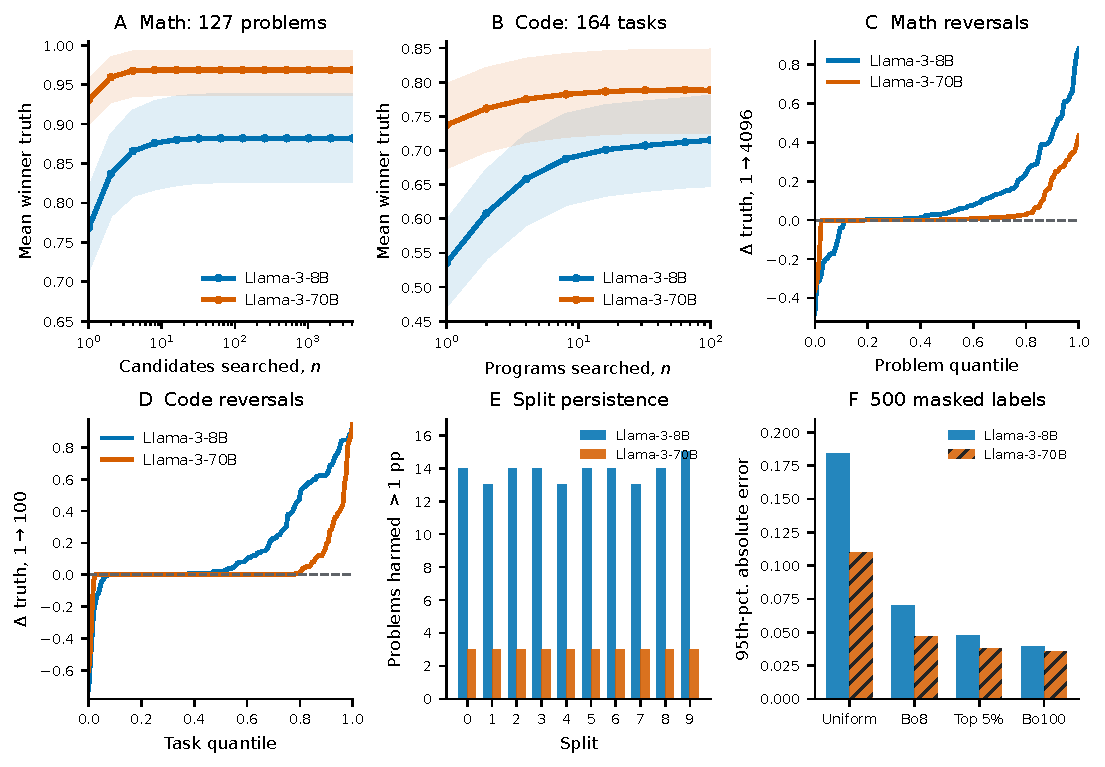
\includegraphics[width=0.98\linewidth]{figures/fig3_empirical_validation_design.pdf}
\caption{\textbf{Retrospective construct checks in two fixed public candidate populations.} (A) Mean selected truth and 95\% problem-bootstrap intervals across 127 GSM8K problems under answer-consensus ranking. (B) The corresponding functional across 164 HumanEval+ tasks under CodeRM ranking. (C,D) Task-level changes include reversals despite favorable aggregate scaling. (E) GSM8K harm counts persist across 10 reference/deployment splits. (F) In masked-label replays at a 500-label budget, a score-tail rule frozen after an 82-task design split reduces held-out best-of-100 estimation error relative to uniform candidate labels. All best-of-$n$ quantities are with-replacement functionals of fixed empirical populations. The panels are not prospective tests of audit effectiveness or prevalence estimates.}
\label{si:fig:empirical-overview}
\end{figure}

\subsection*{S8.1. Dataset and pinning}

The public Monkey Business dataset contains 10,000 generated GSM8K solutions per problem and model \citep{brown2024}. We used 127 problems for each of two configurations:
\begin{itemize}
\item \texttt{GSM8K\_Llama-3-8B-Instruct.json}; SHA-256 \texttt{\seqsplit{0e334c7010a2eb39ab0aaf38cdd196da0b6219a95fd69f82d35b8f51e46ed765}};
\item \texttt{GSM8K\_Llama-3-70B-Instruct.json}; SHA-256 \texttt{\seqsplit{22ff8a363d5a5b8ea5a6c299285d8f615ec32b9c1fe08e8253cc1a6c9c7c323f}}.
\end{itemize}
Both files are downloaded from revision \texttt{a9f8f73bcd6948a57ed922cba4e48062ef95f553}. The pinned release file, rather than an outcome-dependent rule applied by us, fixes the inclusion set: each file contains exactly 127 problem records, and we included every record in both files without excluding any eligible problem. Each record contains 10,000 generated texts and exact final-answer correctness indicators. Total analyzed candidates were $127\times10{,}000\times2=2.54$ million.

\subsection*{S8.2. Consensus score and disjoint deployment population}

Within every model--problem cell, a deterministic random permutation used 2,000 solutions as the reference set and 8,000 as the deployment population. The split seed was 20,260,817 plus fixed model and problem offsets. The final answer following the GSM8K delimiter was normalized by removing commas and whitespace. Its frequency in the reference set was the consensus score for deployment candidates with that answer; unparsable answers received a score below every parsed answer.

For a discrete score group $\ell$, let $F_{\ell-}$ and $F_\ell$ be its lower and upper cumulative population masses and let $t_\ell$ be its mean truth label. Under iid sampling with replacement from the empirical deployment population and uniform tie breaking, the exact selected truth at width $n$ is
\begin{equation}
\widehat\theta_n
=\sum_\ell t_\ell\{F_\ell^n-F_{\ell-}^n\}.
\label{si:eq:empirical-winner}
\end{equation}
This avoids Monte Carlo simulation of search. We evaluated $n\in\{1,2,4,\ldots,4096\}$.

\subsection*{S8.3. Uncertainty and robustness}

All reported aggregates treat the problem as the sampling unit. Percentile intervals use 20,000 bootstrap resamples of the 127 problem rows, with fixed seed 73,041 plus model offset. Macro AUC is the mean within-problem ROC AUC over deployment populations containing both truth classes: 125 problems for Llama-3-8B and 107 for Llama-3-70B. The remaining two and 20 single-class populations remain in all search-reliability and harm summaries but do not have a defined AUC. Ten robustness splits use distinct deterministic seeds and repeat reference scoring, deployment construction, exact winner integration, and harm counting. This checks that reversals are not artifacts of a particular 2,000/8,000 partition; it does not make the 127 GSM8K problems representative of every task domain.

\begin{table}[h]
\centering
\caption{\textbf{Empirical search-scale summary.} Intervals are 95\% problem-bootstrap percentile intervals. Harm counts compare $n=4096$ with $n=1$.}
\label{si:tab:empirical-summary}
\begin{tabular}{lcc}
\toprule
Quantity & Llama-3-8B & Llama-3-70B \\
\midrule
Problems & 127 & 127 \\
Candidates & 1,270,000 & 1,270,000 \\
$\widehat\theta_1$ & 0.7684 & 0.9305 \\
$\widehat\theta_{4096}$ & 0.8819 & 0.9685 \\
Mean change & 0.1135 & 0.0380 \\
Change interval & [0.0748, 0.1538] & [0.0195, 0.0576] \\
Problems entering macro AUC & 125 & 107 \\
Macro AUC & 0.9070 & 0.9617 \\
AUC interval & [0.8616, 0.9474] & [0.9230, 0.9901] \\
Problems harmed $>1$ pp & 14 & 3 \\
Problems harmed $>5$ pp & 12 & 3 \\
Worst problem change & $-0.4796$ & $-0.3598$ \\
Best problem change & 0.8803 & 0.4339 \\
Harm $>1$ pp over 10 splits & 13--15 & 3 in every split \\
\bottomrule
\end{tabular}
\end{table}

These data validate three premises, not the distribution-free worst case itself: the selection kernel changes materially with search breadth; high average rank discrimination can coexist with problem-level reversals; and those reversals persist under resplitting. The Chebyshev theorem is a mathematical identification result and does not require empirical frequency of its extremizers.

\section*{S9. Finite and asymptotic efficiency of validation interventions}

\subsection*{S9.1. Winner-distribution importance sampling}

The target is
\begin{equation}
\theta_N=\int_0^1k_N(u)f(u)du,
\qquad k_N(u)=Nu^{N-1}.
\label{si:eq:eff-target}
\end{equation}
Suppose an audit draws a labeled winner from width $s$, whose percentile density is $q_s(u)=su^{s-1}$. The Horvitz--Thompson variable
\begin{equation}
Z_s=\frac{k_N(U)}{q_s(U)}T,
\qquad U\sim q_s,\quad T\mid U\sim\mathrm{Bernoulli}\{f(U)\},
\label{si:eq:HT}
\end{equation}
is unbiased because
\begin{equation}
\E Z_s=\int q_s\frac{k_N}{q_s}f=\theta_N.
\label{si:eq:HT-unbiased}
\end{equation}
Its second moment is
\begin{align}
\E Z_s^2
&=\int_0^1q_s(u)\left\{\frac{k_N(u)}{q_s(u)}\right\}^2f(u)du\nonumber\\
&=\frac{N^2}{s}\int_0^1u^{2N-s-1}f(u)du\nonumber\\
&=\frac{N^2}{s(2N-s)}\theta_{2N-s},
\label{si:eq:HT-second}
\end{align}
so
\begin{equation}
\operatorname{Var}(Z_s)
=\frac{N^2}{s(2N-s)}\theta_{2N-s}-\theta_N^2.
\label{si:eq:HT-var}
\end{equation}
For $s=N$, the weight is one and the variance is $\theta_N(1-\theta_N)$. We define the variance-equivalent label ratio
\begin{equation}
\rho_s=\frac{\operatorname{Var}(Z_s)}{\theta_N(1-\theta_N)}.
\label{si:eq:ratio}
\end{equation}
Under independent sampling and the same estimator class, $\rho_s$ labels from design $s$ have the same asymptotic variance as one deployment-winner label.

\subsection*{S9.2. Top-tail design}

An audit uniform on the top fraction $a$ of percentiles has density $q_a(u)=a^{-1}\one\{u\ge1-a\}$. It targets the truncated functional
\begin{equation}
\theta_{N,a}=\int_{1-a}^1k_N(u)f(u)du.
\label{si:eq:tail-target}
\end{equation}
The omitted nonnegative mass satisfies
\begin{equation}
0\le\theta_N-\theta_{N,a}
\le\int_0^{1-a}k_N(u)du=(1-a)^N.
\label{si:eq:tail-bias}
\end{equation}
For $a=0.05$ and $N=4096$, this is $0.95^{4096}=5.70\times10^{-92}$. Its importance-weighted second moment is
\begin{equation}
\E Z_a^2
=\frac{aN^2}{2N-1}\theta_{2N-1}^{[1-a,1]},
\label{si:eq:tail-second}
\end{equation}
where the superscript denotes the contribution of the top interval to the corresponding selected-mean integral.

\subsection*{S9.3. Retrospective masked-label acquisition replay}

The variance calculation above predicts a design advantage but does not show its finite-sample size. We therefore used the candidate-level CodeRM data in Section S10 as a label oracle. For every model--task cell, all truth values were treated as masked at the allocation stage. Each acquisition draw first sampled one of the 164 tasks uniformly, then selected a candidate using only its verifier score under one of four fixed rules: uniform candidate, best-of-8 winner, randomized top-5\% score percentile, or best-of-100 deployment winner. Full truth was used only after acquisition to score the estimator against the exact macro best-of-100 target.

For a tied score group occupying sorted candidate indices $a+1,\ldots,b$ among $M=100$ candidates, the probability assigned to each candidate under best-of-$s$ selection is
\begin{equation}
q_s(i)=\frac{(b/M)^s-(a/M)^s}{b-a}.
\label{si:eq:finite-candidate-probability}
\end{equation}
This is exact for with-replacement search, maximum-score selection, and uniform randomization within the winning tie. Let $p_i=q_{100}(i)$ denote the target probability and let $q_i$ denote the audit probability within the sampled task. The revealed-label variable
\begin{equation}
Z_i=\frac{p_i}{q_i}T_i,
\label{si:eq:finite-HT}
\end{equation}
is unbiased for the task-averaged best-of-100 target whenever $q_i>0$ wherever $p_i>0$. For the top-tail design, Eq.~\ref{si:eq:finite-HT} estimates the truncated target; the missing mass is at most $0.95^{100}=0.0059205$. Randomized percentile sampling distributes a boundary-crossing tie uniformly across the entire score group.

We ran 5,000 independent acquisition replicates for label budgets $25,50,100,250,500,1{,}000,2{,}000,$ and $5{,}000$, using seed 131,071 plus fixed model and design offsets. Within a replicate, samples accumulate across budgets. The primary finite error metric is the 95th percentile across replicates of $|\widehat\theta_{100}-\theta_{100}|$; root mean squared and median absolute errors are also written to \texttt{results/coderm\_label\_acquisition.csv}.

\begin{table}[h]
\centering
\caption{\textbf{Finite masked-label error for best-of-100 CodeRM truth.} Entries are the 95th percentile of absolute error across 5,000 retrospective replays. Allocation uses scores only; full labels score the emulation afterward.}
\label{si:tab:finite-label-acquisition}
\begin{tabular}{llrrrr}
\toprule
Model & Audit design & 100 & 500 & 1,000 & 5,000 labels \\
\midrule
8B & Uniform candidate & 0.444 & 0.184 & 0.131 & 0.060 \\
8B & Best-of-8 winner & 0.157 & 0.070 & 0.051 & 0.022 \\
8B & Top-5\% percentile & 0.105 & 0.047 & 0.034 & 0.015 \\
8B & Best-of-100 winner & 0.085 & 0.039 & 0.028 & 0.013 \\
70B & Uniform candidate & 0.212 & 0.110 & 0.079 & 0.035 \\
70B & Best-of-8 winner & 0.109 & 0.047 & 0.033 & 0.015 \\
70B & Top-5\% percentile & 0.085 & 0.038 & 0.027 & 0.012 \\
70B & Best-of-100 winner & 0.082 & 0.036 & 0.025 & 0.011 \\
\bottomrule
\end{tabular}
\end{table}

At 500 labels, replacing uniform acquisition by the top-tail design reduced the 95th-percentile error by factors 3.89 and 2.89 for 8B and 70B. The same top-5\% rule, budgets, and estimator were used for both models; no model-specific truth information changes allocation. The actual top-tail truncation biases under the fully labeled empirical populations were $9.75\times10^{-5}$ and $3.64\times10^{-5}$, far below the distribution-free bound, but those empirical values are used only for retrospective scoring. This is a finite label-acquisition emulation, not a prospective experiment with newly generated candidates or newly collected truths. A genuinely prospective test would randomize the audit design before outcomes are produced and should additionally account for per-design generation cost.

The replay errors and the 1,000-bin feasible spans in Section S10.2 are not one metric. The prefix programs construct compatible continuum step-function witnesses under exact or banded mean constraints; the replay asks how a fixed estimator behaves when labels are acquired in different score directions. Their joint conclusion is narrower than a prospective effectiveness claim: on the same best-of-100 functional, covered search widths, independent task count, and label direction address different failure modes and must be planned separately.

\subsection*{S9.4. Frozen-rule held-out audit test}

The full-pool replay above fixes the allocation rule in advance but evaluates it on the same task population used to report the comparison. To test whether an audit rule selected from data transfers across tasks, we added a label-blind discovery/held-out split before examining outcomes. With seed 260,821, the 164 task identifiers shared by both CodeRM models were permuted once and divided into 82 discovery and 82 held-out tasks. The split is shared across models and is recorded in \texttt{results/coderm\_heldout\_task\_split.csv}.

The candidate audit family was fixed at the top 5\%, 10\%, or 20\% of score percentiles. All three designs leave at most $0.95^{100}=0.0059205$ of the best-of-100 target mass unsupported. On discovery tasks only, we ran 5,000 masked-label replays at a budget of 500 and selected the fraction minimizing the mean 95th-percentile absolute error across the two models. Mean discovery errors were $0.0427$, $0.0546$, and $0.0751$, respectively, so the 5\% rule was selected. That rule was then frozen before the held-out target and replay error were computed. Uniform acquisition served as the held-out comparator. The estimator and exact tied-score candidate probabilities are those in Eqs.~\ref{si:eq:finite-candidate-probability} and \ref{si:eq:finite-HT}; independent replay streams use seed 262,147 plus fixed design and model offsets.

\begin{table}[h]
\centering
\caption{\textbf{Frozen-rule performance on 82 held-out CodeRM tasks.} Entries are based on 5,000 retrospective masked-label replays at 500 labels. The top-tail fraction was chosen on a disjoint 82-task discovery split and frozen before held-out outcomes were scored.}
\label{si:tab:heldout-audit}
\begin{tabular}{lrrrr}
\toprule
Model & Held-out target & Uniform q95 error & Frozen top-5\% q95 error & Frozen absolute bias \\
\midrule
8B & 0.698 & 0.180 & 0.049 & $7.58\times10^{-5}$ \\
70B & 0.791 & 0.076 & 0.035 & $7.28\times10^{-5}$ \\
\bottomrule
\end{tabular}
\end{table}

The frozen rule reduced the held-out q95 error by factors 3.67 and 2.15. This is stronger than selecting and evaluating a design on the same task set: held-out outcomes did not choose the tail fraction. It is nevertheless not a prospective intervention. Both splits come from one existing public dataset, all candidates and labels had already been generated, and the replay does not measure collection cost, distribution shift, or a causal effect of assigning a real evaluation program. Complete discovery and held-out metrics, including median error and RMSE, are in \texttt{results/coderm\_heldout\_audit.csv}.

\subsection*{S9.5. Asymptotic GSM8K calculation}

Within each model, tie-averaged truth was aggregated into 20 equal-width percentile bins across problems. Treating the bin means as a piecewise-constant $f$, all moments in Eqs.~\ref{si:eq:HT-var} and \ref{si:eq:tail-second} are analytic differences of bin-edge powers. This binning is deliberately coarse; at $N=4096$, essentially all target mass lies in the last bin, and the computation is a transparent design comparison rather than a claim of nonparametric tail recovery.

\begin{table}[h]
\centering
\caption{\textbf{Variance-equivalent labels for a best-of-4096 target.} Each entry is the number of labels under the row design needed to match the asymptotic variance of one deployment-winner label.}
\label{si:tab:efficiency}
\begin{tabular}{lrr}
\toprule
Audit design & Llama-3-8B & Llama-3-70B \\
\midrule
Uniform candidate & 17,333.7 & 64,993.0 \\
Best-of-8 winner & 2,162.0 & 8,104.2 \\
Best-of-64 winner & 265.6 & 993.1 \\
Uniform top 5\% rank & 859.6 & 3,220.4 \\
Best-of-4096 winner & 1.0 & 1.0 \\
\bottomrule
\end{tabular}
\end{table}

The large ratios have a simple source. Under uniform candidate sampling, the importance weight near $u=1$ is approximately $N$, so rare tail labels receive enormous leverage. The deployment-winner design samples directly from that tail and uses unit weights. The ratios depend on $f$, $N$, the score law, and the estimator; they are not transferable constants. In a real evaluation, cost per label, dependence among generated candidates, and the feasibility of producing deployment winners must also be included.

\subsection*{S9.6. Prospective intervention specification}

The public-data experiment can be converted into a genuinely prospective test without changing its estimand. Before generating or labeling new outcomes, register the target width $N$, task population, verifier, tie rule, label budget, top-tail fraction, and the uniform-versus-score-matched allocation comparison. Randomize independent task--model cells to audit designs before truth is observed; retain the task as the cluster; and collect a fully labeled evaluation subset only to score estimator error, not to choose the allocation. The primary comparison should be finite-sample squared or absolute error at a fixed total cost, with coverage and generation cost as secondary outcomes. If the objective is instead a distribution-free direct-winner interval of full width $0.10$ at 95\% confidence, Eq.~\ref{si:eq:direct-task-count} requires 738 independent tasks; this is a conservative certificate calculation, not a power analysis. The fixed replay design used here---$N=100$, top 5\%, and the eight reported budgets---is a ready specification, but this paragraph is a protocol, not additional prospective evidence.

\section*{S10. Code-generation replication and reproducibility}

\subsection*{S10.1. CodeRM/HumanEval+ data and estimand}

The independent domain is the public CodeRM release \citep{ma2025}, pinned at Git commit \texttt{\seqsplit{aa4946e9245ed41e24d60ad29e965132b5b84fe6}}. We used all 164 HumanEval+ tasks and the first 100 candidate programs per task from each of the Llama-3-8B and Llama-3-70B annotated solution files. The annotation SHA-256 digests are, respectively,
\begin{itemize}
\item \texttt{\seqsplit{cae513c7578a52c6d3110a13bbf2514e44a0cd58f2a4a258b58e7337c2af0211}};
\item \texttt{\seqsplit{6ddb4273e4d9a35f7bef6016f37ac2e9b99d6bd7aad05357f7ff9399b0d45850}}.
\end{itemize}
Objective truth is the HumanEval+ \texttt{plus\_status} field, which evaluates the program against the benchmark's expanded hidden tests.

The CodeRM output archive linked by the repository README has SHA-256
\texttt{728780d642f465e9}\allowbreak\texttt{1f8619de1bae0cb3}\allowbreak\texttt{192519278e87014d}\allowbreak\texttt{546cee9921d4e6c5}. For each model we used the public 100-solution by 100-generated-unit-test execution matrix. The extracted JSONL member digests are
\begin{itemize}
\item 8B: \texttt{\seqsplit{8169be74c8144e0bad6b593093a02e4963144f66a6a5f6b84c10ff1dd6e316d1}};
\item 70B: \texttt{\seqsplit{7edb5fc98033f5de748c5dfe2f740cdeffb02020ead8f49988ea822d2d8d2fdf}}.
\end{itemize}
For candidate $i$, the verifier score is the fraction of the 100 CodeRM-8B-generated unit tests for which the execution result is \texttt{pass}. The data therefore contain $164\times100\times2=32{,}800$ programs and $3.28$ million candidate--test executions. The generated tests determine ranking; the distinct HumanEval+ status determines truth.

Within each model--task cell, Eq.~\ref{si:eq:empirical-winner} was applied to the empirical verifier-score groups, with exact uniform tie breaking, for $n\in\{1,2,4,8,16,32,64,100\}$. Intervals use 20,000 task bootstrap resamples, with seed 92,771 plus model offset. AUC gives half credit to tied positive--negative pairs. All 164 tasks contain both truth classes for each model and therefore enter both macro AUCs. The task is the independent unit; the 100 generated tests do not count as 100 independent benchmark tasks.

\begin{table}[h]
\centering
\caption{\textbf{Independent CodeRM/HumanEval+ replication.} Intervals are 95\% task-bootstrap percentile intervals. Harm compares best-of-100 with one random program.}
\label{si:tab:coderm-summary}
\begin{tabular}{lcc}
\toprule
Quantity & Llama-3-8B & Llama-3-70B \\
\midrule
Tasks & 164 & 164 \\
Candidate programs & 16,400 & 16,400 \\
Candidate--test executions & 1,640,000 & 1,640,000 \\
Tasks entering macro AUC & 164 & 164 \\
Macro AUC & 0.931 [0.898, 0.959] & 0.881 [0.818, 0.938] \\
$\widehat\theta_1$ & 0.536 [0.473, 0.597] & 0.737 [0.675, 0.797] \\
$\widehat\theta_{100}$ & 0.715 [0.649, 0.780] & 0.788 [0.726, 0.847] \\
Mean change & 0.179 [0.134, 0.226] & 0.051 [0.025, 0.080] \\
Tasks harmed by $>1$ pp & 10 & 4 \\
Worst task change & $-0.722$ & $-0.600$ \\
\bottomrule
\end{tabular}
\end{table}

The CodeRM replication is not a second estimate of the GSM8K mechanism. It deliberately changes the domain, generator outputs, score construction, truth mechanism, and search range. Its role is to test the more basic prediction that a favorable average verifier can induce a heterogeneous reliability spectrum with severe local reversals. The repository did not expose an explicit license file at the pinned revision, so the package does not redistribute programs, generated unit tests, or execution logs. It includes only derived numeric candidate scores and labels, plus a checksum-verifying reconstruction script.

\subsection*{S10.2. Retrospective compatibility from an audited prefix}

The main-text certification exercise uses the same 32,800 derived CodeRM score--truth rows. Within task $t$, sort the 100 candidates by verifier score. If a score-tie group occupies percentile intervals $I_{tj}$ and has mean truth $\bar T_{tj}$, define the bounded step function
\begin{equation}
\widehat f_t(u)=\bar T_{tj},\qquad u\in I_{tj}.
\label{si:eq:task-rank-law}
\end{equation}
Spreading a tie group's mean over its occupied intervals is exactly equivalent to uniform tie breaking. Consequently the macro law $\widehat f=164^{-1}\sum_t\widehat f_t$ satisfies
\begin{equation}
\int_0^1nu^{n-1}\widehat f(u)\,du
=\frac1{164}\sum_{t=1}^{164}\widehat\theta_{t,n}
\label{si:eq:macro-rank-law}
\end{equation}
for every integer $n$, not only for the eight search widths previously plotted.

To ask what the audited prefix alone certifies, refine the 100 empirical rank intervals to $J=1{,}000$ equal bins and let $g_j\in[0,1]$ be a candidate law on bin $j$. Put
\begin{equation}
w_{n,j}=\left(\frac jJ\right)^n-\left(\frac{j-1}J\right)^n.
\label{si:eq:bin-mass}
\end{equation}
For each $m$, the plug-in endpoints solve the two linear programs
\begin{equation}
\underset{0\le g\le1}{\operatorname{minimize/maximize}}\quad
w_N^\top g
\quad\text{subject to}\quad
w_n^\top g=\widehat\theta_n,\quad n=1,\ldots,m.
\label{si:eq:empirical-partial-id-lp}
\end{equation}
Every optimizer defines a bounded piecewise-constant function on $[0,1]$. Thus the displayed separation is a constructive lower bound on the unrestricted continuum identified width; it is not created by allowing infeasible grid vectors. Raw power-moment rows become nearly collinear as $m$ grows. For exact plug-in equalities, the implementation therefore normalizes the rows and replaces them by an orthonormal basis obtained from a QR factorization of the transposed audit matrix. This changes neither the row space nor the exact feasible set, but prevents a tiny raw-moment tolerance from becoming a large extrapolated target error. At $m=8$, increasing $J$ from 200 to 500 and 1,000 changed every endpoint by less than $0.007$. The maximum raw equality residual at $J=1{,}000$ was $1.3\times10^{-14}$.

Finite task sampling uncertainty was propagated separately. We drew 20,000 multinomial bootstrap resamples of the 164 tasks. For each $m$, let $\widehat s_n$ be the bootstrap standard error and let $c_m$ be the 95th percentile of
\begin{equation}
\max_{1\le n\le m}
\left|\frac{\widehat\theta_n^*-\widehat\theta_n}{\widehat s_n}\right|.
\label{si:eq:max-t-band}
\end{equation}
Replacing the equalities in Eq.~\ref{si:eq:empirical-partial-id-lp} by the simultaneous inequalities
$\widehat\theta_n-c_m\widehat s_n\le w_n^\top g\le\widehat\theta_n+c_m\widehat s_n$, truncated to $[0,1]$, gives the bootstrap-feasible ranges in Table~\ref{si:tab:partial-id}. They condition on the empirical score/rank construction and use the task as the sampling unit; they are not a distribution-shift guarantee.

\begin{table}[h]
\centering
\caption{\textbf{CodeRM best-of-100 ranges from audits through $m$.} Plug-in columns impose exact empirical means at every integer $n\le m$. Bootstrap columns allow the simultaneous 95\% task-bootstrap band. Observed best-of-100 truth is 0.715 for 8B and 0.788 for 70B.}
\label{si:tab:partial-id}
\begin{tabular}{lrrcc}
\toprule
Model & $m$ & Plug-in range & Width & Bootstrap-feasible range \\
\midrule
Llama-3-8B  & 4  & [0.003, 1.000] & 0.997 & [0.000, 1.000] \\
             & 8  & [0.186, 0.992] & 0.806 & [0.003, 1.000] \\
             & 12 & [0.453, 0.907] & 0.453 & [0.021, 1.000] \\
             & 16 & [0.620, 0.796] & 0.176 & [0.056, 1.000] \\
             & 20 & [0.690, 0.737] & 0.047 & [0.102, 0.999] \\
\midrule
Llama-3-70B & 4  & [0.018, 1.000] & 0.982 & [0.000, 1.000] \\
             & 8  & [0.305, 0.996] & 0.691 & [0.016, 1.000] \\
             & 12 & [0.569, 0.937] & 0.367 & [0.065, 1.000] \\
             & 16 & [0.711, 0.852] & 0.141 & [0.130, 1.000] \\
             & 20 & [0.769, 0.806] & 0.038 & [0.197, 1.000] \\
\bottomrule
\end{tabular}
\end{table}

\begin{figure}[h]
\centering
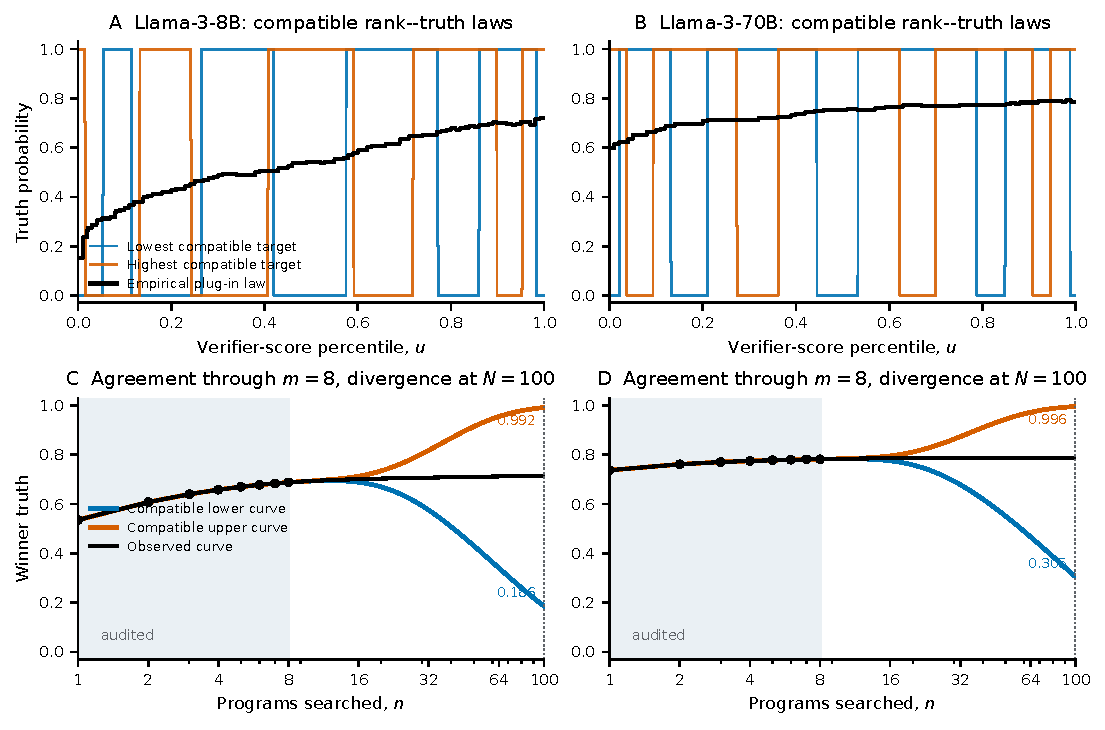
\includegraphics[width=0.95\linewidth]{figures/fig4_empirical_partial_identification.pdf}
\caption{\textbf{An empirical audited prefix does not certify the deployment target.} (A,B) For each CodeRM model, linear programs construct bounded piecewise-constant rank--truth laws that match the empirical best-of-$n$ means for every $n=1,\ldots,8$ while minimizing or maximizing best-of-100 truth; the black line is the empirical plug-in law. (C,D) The induced search curves coincide throughout the shaded audited range and then separate. At $N=100$, the constructive plug-in ranges are $[0.186,0.992]$ for 8B and $[0.305,0.996]$ for 70B; observed values are $0.715$ and $0.788$. The grid laws are feasible continuum laws, so their separation is a witnessed lower bound on unrestricted empirical ambiguity.}
\label{si:fig:partialid}
\end{figure}

The $m=8$ extremizers are plotted in Fig.~\ref{si:fig:partialid}. They are not fitted forecasts of best-of-100 truth; they are witnesses to nonidentification. The observed target lies inside every reported range, as it must because the empirical rank--truth law itself is feasible. Machine-readable endpoints, bootstrap critical values, grid checks, and all 1,000-bin extremizers are supplied in \texttt{results/coderm\_partial\_identification.csv}, \texttt{results/coderm\_partial\_id\_grid\_check.csv}, and \texttt{results/coderm\_partial\_id\_worlds.csv}.

\subsection*{S10.3. Independent theorem checks}

For $m=1,\ldots,8$ and four values of $N$ per $m$, the reproducibility script performed three independent computations:
\begin{enumerate}
\item evaluated the closed form in Eq.~\ref{si:eq:closed-form};
\item constructed the barycentric interpolant at the $U_m$ roots and integrated its absolute error by adaptive quadrature split at every root;
\item integrated $u^k\sigma_m(u)$ for $k=0,\ldots,m-1$ to check audited-moment annihilation.
\end{enumerate}
Across 32 cases, the largest absolute difference between items 1 and 2 was $1.887\times10^{-15}$. The largest absolute residual in item 3 was $3.331\times10^{-16}$.

\begin{table}[h]
\centering
\caption{\textbf{Representative exact-frontier checks.} The complete 32-row table is \texttt{results/theorem\_checks.csv}.}
\label{si:tab:checks}
\begin{tabular}{rrrrr}
\toprule
$m$ & $N$ & Closed form & Quadrature & Max moment residual \\
\midrule
1 & 16 & 0.9999694824 & 0.9999694824 & 0 \\
2 & 21 & 0.9952431821 & 0.9952431821 & $2.22\times10^{-16}$ \\
4 & 31 & 0.9109153208 & 0.9109153208 & $4.16\times10^{-17}$ \\
6 & 41 & 0.7510560990 & 0.7510560990 & $3.33\times10^{-16}$ \\
8 & 51 & 0.5838695161 & 0.5838695161 & $1.11\times10^{-16}$ \\
\bottomrule
\end{tabular}
\end{table}

The numerical checks are not substitutes for the proof. They are designed to detect sign, indexing, interpolation-node, and phase-scaling errors in the implementation.

\subsection*{S10.4. Reproduction workflow}

The package contains:
\begin{itemize}
\item \texttt{code/reproduce\_geometry\_validation.py}: unrestricted and shape-restricted theorem checks, phase and finite-certificate planning tables, CodeRM reconstruction from derived numbers, QR-stabilized empirical partial-identification programs, finite masked-label acquisition, the frozen-rule discovery/held-out audit, Gaussian selection, intervention efficiency, and all deterministic figures;
\item \texttt{code/solve\_capped\_tail\_dual.py}: nested-bin primal--dual LPs, continuum scalar-threshold evaluation, optimizer coefficients, and percentile-scale $L$ sensitivity;
\item \texttt{code/analyze\_search\_spectrum.py}: pinned raw-data download, checksum verification, reference/deployment analysis, bootstrap, and processed tables;
\item \texttt{code/analyze\_split\_robustness.py}: the 10-split robustness analysis;
\item \texttt{code/analyze\_coderm\_search.py}: CodeRM checksum verification, streaming execution-matrix aggregation, exact search curves, task bootstrap, and derived candidate table;
\item \texttt{data/processed/}: exact processed inputs, including 32,800 derived CodeRM score--truth rows, used by the lightweight reproduction;
\item \texttt{results/}: machine-readable unrestricted and regularized theorem bounds, capped-tail primal--dual checks and optimizers, phase, finite certificate plans, Gaussian, CodeRM, partial-identification extremizers and grid checks, finite label-acquisition errors, discovery/held-out task assignments and errors, and design-efficiency outputs.
\end{itemize}
The lightweight script requires Python 3.12, NumPy, SciPy, and Matplotlib and does not download data or call a model API. The full GSM8K reconstruction additionally uses scikit-learn and downloads the two pinned raw files (approximately 18.5 GB combined). The CodeRM reconstruction reads the public 213-MB compressed output archive and the pinned annotation files. Every figure is deterministic. Bootstrap seeds are stated above; analytic theorem figures do not rely on Monte Carlo draws.

\section*{S11. Relation to adjacent literatures and contribution boundary}

The mathematical ingredients have substantial precedents. The audit prefix is
a truncated Hausdorff moment problem: classical work characterizes feasible
moment sequences, while canonical-moment and Tchebycheff-system theory studies
the geometry and extremal representations of the resulting moment spaces
\citep{hausdorff1921,dette1997}. Once $k_1,\ldots,k_m$ are recognized to span
$\mathcal P_{m-1}$, optimal-recovery duality and canonical $L^1$
approximation give the unrestricted distance \citep{donoho1994,bojanov1986}.
Bounded-density moment theory supplies feasibility characterizations for the
Lipschitz derivative measure \citep{lasserre2006}. The submitted objects are
the diameters and residual support functionals induced by the stated
best-of-$N$ audit/deployment kernels after imposing bounded reliability,
monotonicity, or a density cap. No general theorem about moment spaces,
canonical representations, quotient duality, orthogonal polynomials, or
moment representation is claimed as new.

Two close AI results mark the applied boundary. \emph{ROC-n-reroll} gives
verifiers with arbitrarily close finite best-of-$N$ behavior and opposite
infinite-compute limits \citep{dorner2026}, whereas the present unrestricted
benchmark requires exact prefix equality and solves a specified finite target.
\emph{Evaluation Blind Spot} studies geometric recovery for static benchmark
coverage \citep{wang2026}; the object here is selected-output truth under an
explicit deployment kernel. These distinctions delimit the submitted object.

Closer statistical neighbors are Mallows's parent-distribution bounds from
expected order statistics \citep{mallows1973}, Papadatos's expected-maxima and
range sequences \citep{papadatos2017}, and Okolewski and Papadatos's finite
expected-order-statistic/truncated-moment connection \citep{okolewski2024}.
They clarify feasibility and recovery. To our knowledge, they do not state the
bounded-binary exact interval for a best-of-width reliability prefix, its
low-width reliability-mean maximality, or the monotone and capped-Lipschitz
residuals stated here. Huang et al. instead study coverage and optimal alignment
under imperfect rewards \citep{huang2025}. Accordingly, the contribution claimed
here is the exact validation object and its consequences, not a new
characterization of expected order statistics.

\subsection*{S11.1. Theorem-by-theorem provenance}

Table~\ref{si:tab:provenance} gives the theorem-level boundary. Classical moment, approximation, and bounded-density results supply the mathematical ingredients \citep{hausdorff1921,dette1997,bojanov1986,newman1976,lasserre2006}; finite expected-order-statistic work supplies the closest statistical representation results \citep{mallows1973,papadatos2017,okolewski2024}; and recent best-of-$N$ theory supplies the closest AI decision setting \citep{huang2025}. The third column states the remaining validation-specific contribution.

\begin{table}[H]
\centering
\caption{\textbf{Concise contribution boundary.} ``Submitted object'' is validation-specific; the listed mathematical tools are established inputs.}
\label{si:tab:provenance}
\begingroup
\footnotesize
\setlength{\tabcolsep}{3pt}
\begin{tabular}{@{}>{\raggedright\arraybackslash}p{0.22\linewidth}>{\raggedright\arraybackslash}p{0.34\linewidth}>{\raggedright\arraybackslash}p{0.38\linewidth}@{}}
\toprule
Result & Classical input & Submitted object \\
\midrule
Unrestricted benchmark & Hausdorff/canonical moment spaces \citep{hausdorff1921,dette1997}, quotient recovery \citep{donoho1994}, and canonical $L^1$ approximation \citep{bojanov1986} & Full bounded binary identified interval, attainable endpoints and interior laws, plus the finite theta phase law \\
Monotone frontier & Measure representation and uniform monomial approximation \citep{newman1976} & Exact reduction of compatible monotone validation worlds to $2E_m(u^N)$ \\
Monotone Lipschitz frontier & Compact measure duality and bounded-density moments \citep{lasserre2006} & Exact capped-tail residual dual for the stated validation kernels \\
Endpoint bounds & Legendre orthogonality, Gauss recovery, and extreme-zero asymptotics & Explicit smooth compatible worlds and order-sharp fixed-$L$ bounds \\
Scope and sampling & Span inclusion, concentration, and perturbation inequalities \citep{ettehad2021} & Width coverage separated from task precision; no new abstract recovery or concentration theorem is claimed \\
\bottomrule
\end{tabular}
\endgroup
\end{table}

\subsection*{S11.2. Exact claim}

The submitted claim is that the specified validation and deployment kernels
produce the exact attainable identification objects in
Table~\ref{si:tab:provenance}, including the monotone and capped-Lipschitz duals,
the reliability-mean audit law, and the finite planning consequences. No general
inverse-problem, moment, order-statistic, approximation, orthogonal-polynomial,
or theta-function theorem is claimed. Complete proofs are given in Sections
S1--S7, with executable numerical checks for every reported finite calculation.

The empirical role is narrower. Independent units are 127 problems and 164
tasks; candidate outputs repeat within them. The analyses show target change,
reversals, compatible witnesses, and a within-pool acquisition contrast, not
prevalence, extremal-world frequency, or prospective effectiveness. The 82/82
split protects held-out labels from rule selection but remains a public-data
replay.
